
%% bare_jrnl_compsoc.tex
%% V1.4a
%% 2014/09/17
%% by Michael Shell
%% See:
%% http://www.michaelshell.org/
%% for current contact information.
%%
%% This is a skeleton file demonstrating the use of IEEEtran.cls
%% (requires IEEEtran.cls version 1.8a or later) with an IEEE
%% Computer Society journal paper.
%%
%% Support sites:
%% http://www.michaelshell.org/tex/ieeetran/
%% http://www.ctan.org/tex-archive/macros/latex/contrib/IEEEtran/
%% and
%% http://www.ieee.org/

%%*************************************************************************
%% Legal Notice:
%% This code is offered as-is without any warranty either expressed or
%% implied; without even the implied warranty of MERCHANTABILITY or
%% FITNESS FOR A PARTICULAR PURPOSE!
%% User assumes all risk.
%% In no event shall IEEE or any contributor to this code be liable for
%% any damages or losses, including, but not limited to, incidental,
%% consequential, or any other damages, resulting from the use or misuse
%% of any information contained here.
%%
%% All comments are the opinions of their respective authors and are not
%% necessarily endorsed by the IEEE.
%%
%% This work is distributed under the LaTeX Project Public License (LPPL)
%% ( http://www.latex-project.org/ ) version 1.3, and may be freely used,
%% distributed and modified. A copy of the LPPL, version 1.3, is included
%% in the base LaTeX documentation of all distributions of LaTeX released
%% 2003/12/01 or later.
%% Retain all contribution notices and credits.
%% ** Modified files should be clearly indicated as such, including  **
%% ** renaming them and changing author support contact information. **
%%
%% File list of work: IEEEtran.cls, IEEEtran_HOWTO.pdf, bare_adv.tex,
%%                    bare_conf.tex, bare_jrnl.tex, bare_conf_compsoc.tex,
%%                    bare_jrnl_compsoc.tex, bare_jrnl_transmag.tex
%%*************************************************************************


% *** Authors should verify (and, if needed, correct) their LaTeX system  ***
% *** with the testflow diagnostic prior to trusting their LaTeX platform ***
% *** with production work. IEEE's font choices and paper sizes can       ***
% *** trigger bugs that do not appear when using other class files.       ***                          ***
% The testflow support page is at:
% http://www.michaelshell.org/tex/testflow/


\documentclass[10pt,journal]{IEEEtran}
\usepackage{savesym}
\usepackage{amsmath}
\savesymbol{iint}
\usepackage{txfonts}
\usepackage{graphicx}
%\usepackage{amssymb}
%\usepackage{verbatim}
\usepackage{algorithm} %format of the algorithm
\usepackage{algorithmic}
%\usepackage{algorithmic2e}
\usepackage{subfigure}
\usepackage{multirow}
\usepackage{epstopdf}
% If IEEEtran.cls has not been installed into the LaTeX system files,
% manually specify the path to it like:
% \documentclass[10pt,journal,compsoc]{../sty/IEEEtran}


\newtheorem{definition}{\textbf{Definition}}
\newtheorem{lemma}{\textbf{Lemma}}
\newtheorem{property}{\textbf{Property}}
\newtheorem{proof}{Proof}
\newtheorem{problem}{\textbf{Problem}}



\hyphenpenalty=7000


% Some very useful LaTeX packages include:
% (uncomment the ones you want to load)


% *** MISC UTILITY PACKAGES ***
%
%\usepackage{ifpdf}
% Heiko Oberdiek's ifpdf.sty is very useful if you need conditional
% compilation based on whether the output is pdf or dvi.
% usage:
% \ifpdf
%   % pdf code
% \else
%   % dvi code
% \fi
% The latest version of ifpdf.sty can be obtained from:
% http://www.ctan.org/tex-archive/macros/latex/contrib/oberdiek/
% Also, note that IEEEtran.cls V1.7 and later provides a builtin
% \ifCLASSINFOpdf conditional that works the same way.
% When switching from latex to pdflatex and vice-versa, the compiler may
% have to be run twice to clear warning/error messages.






% *** CITATION PACKAGES ***
%
\ifCLASSOPTIONcompsoc
  % IEEE Computer Society needs nocompress option
  % requires cite.sty v4.0 or later (November 2003)
  \usepackage[nocompress]{cite}
\else
  % normal IEEE
  \usepackage{cite}
\fi
% cite.sty was written by Donald Arseneau
% V1.6 and later of IEEEtran pre-defines the format of the cite.sty package
% \cite{} output to follow that of IEEE. Loading the cite package will
% result in citation numbers being automatically sorted and properly
% "compressed/ranged". e.g., [1], [9], [2], [7], [5], [6] without using
% cite.sty will become [1], [2], [5]--[7], [9] using cite.sty. cite.sty's
% \cite will automatically add leading space, if needed. Use cite.sty's
% noadjust option (cite.sty V3.8 and later) if you want to turn this off
% such as if a citation ever needs to be enclosed in parenthesis.
% cite.sty is already installed on most LaTeX systems. Be sure and use
% version 5.0 (2009-03-20) and later if using hyperref.sty.
% The latest version can be obtained at:
% http://www.ctan.org/tex-archive/macros/latex/contrib/cite/
% The documentation is contained in the cite.sty file itself.
%
% Note that some packages require special options to format as the Computer
% Society requires. In particular, Computer Society  papers do not use
% compressed citation ranges as is done in typical IEEE papers
% (e.g., [1]-[4]). Instead, they list every citation separately in order
% (e.g., [1], [2], [3], [4]). To get the latter we need to load the cite
% package with the nocompress option which is supported by cite.sty v4.0
% and later. Note also the use of a CLASSOPTION conditional provided by
% IEEEtran.cls V1.7 and later.





% *** GRAPHICS RELATED PACKAGES ***
%
\ifCLASSINFOpdf
  % \usepackage[pdftex]{graphicx}
  % declare the path(s) where your graphic files are
  % \graphicspath{{../pdf/}{../jpeg/}}
  % and their extensions so you won't have to specify these with
  % every instance of \includegraphics
  % \DeclareGraphicsExtensions{.pdf,.jpeg,.png}
\else
  % or other class option (dvipsone, dvipdf, if not using dvips). graphicx
  % will default to the driver specified in the system graphics.cfg if no
  % driver is specified.
  % \usepackage[dvips]{graphicx}
  % declare the path(s) where your graphic files are
  % \graphicspath{{../eps/}}
  % and their extensions so you won't have to specify these with
  % every instance of \includegraphics
  % \DeclareGraphicsExtensions{.eps}
\fi
% graphicx was written by David Carlisle and Sebastian Rahtz. It is
% required if you want graphics, photos, etc. graphicx.sty is already
% installed on most LaTeX systems. The latest version and documentation
% can be obtained at:
% http://www.ctan.org/tex-archive/macros/latex/required/graphics/
% Another good source of documentation is "Using Imported Graphics in
% LaTeX2e" by Keith Reckdahl which can be found at:
% http://www.ctan.org/tex-archive/info/epslatex/
%
% latex, and pdflatex in dvi mode, support graphics in encapsulated
% postscript (.eps) format. pdflatex in pdf mode supports graphics
% in .pdf, .jpeg, .png and .mps (metapost) formats. Users should ensure
% that all non-photo figures use a vector format (.eps, .pdf, .mps) and
% not a bitmapped formats (.jpeg, .png). IEEE frowns on bitmapped formats
% which can result in "jaggedy"/blurry rendering of lines and letters as
% well as large increases in file sizes.
%
% You can find documentation about the pdfTeX application at:
% http://www.tug.org/applications/pdftex






% *** MATH PACKAGES ***
%
%\usepackage[cmex10]{amsmath}
% A popular package from the American Mathematical Society that provides
% many useful and powerful commands for dealing with mathematics. If using
% it, be sure to load this package with the cmex10 option to ensure that
% only type 1 fonts will utilized at all point sizes. Without this option,
% it is possible that some math symbols, particularly those within
% footnotes, will be rendered in bitmap form which will result in a
% document that can not be IEEE Xplore compliant!
%
% Also, note that the amsmath package sets \interdisplaylinepenalty to 10000
% thus preventing page breaks from occurring within multiline equations. Use:
%\interdisplaylinepenalty=2500
% after loading amsmath to restore such page breaks as IEEEtran.cls normally
% does. amsmath.sty is already installed on most LaTeX systems. The latest
% version and documentation can be obtained at:
% http://www.ctan.org/tex-archive/macros/latex/required/amslatex/math/





% *** SPECIALIZED LIST PACKAGES ***
%
%\usepackage{algorithmic}
% algorithmic.sty was written by Peter Williams and Rogerio Brito.
% This package provides an algorithmic environment fo describing algorithms.
% You can use the algorithmic environment in-text or within a figure
% environment to provide for a floating algorithm. Do NOT use the algorithm
% floating environment provided by algorithm.sty (by the same authors) or
% algorithm2e.sty (by Christophe Fiorio) as IEEE does not use dedicated
% algorithm float types and packages that provide these will not provide
% correct IEEE style captions. The latest version and documentation of
% algorithmic.sty can be obtained at:
% http://www.ctan.org/tex-archive/macros/latex/contrib/algorithms/
% There is also a support site at:
% http://algorithms.berlios.de/index.html
% Also of interest may be the (relatively newer and more customizable)
% algorithmicx.sty package by Szasz Janos:
% http://www.ctan.org/tex-archive/macros/latex/contrib/algorithmicx/




% *** ALIGNMENT PACKAGES ***
%
%\usepackage{array}
% Frank Mittelbach's and David Carlisle's array.sty patches and improves
% the standard LaTeX2e array and tabular environments to provide better
% appearance and additional user controls. As the default LaTeX2e table
% generation code is lacking to the point of almost being broken with
% respect to the quality of the end results, all users are strongly
% advised to use an enhanced (at the very least that provided by array.sty)
% set of table tools. array.sty is already installed on most systems. The
% latest version and documentation can be obtained at:
% http://www.ctan.org/tex-archive/macros/latex/required/tools/


% IEEEtran contains the IEEEeqnarray family of commands that can be used to
% generate multiline equations as well as matrices, tables, etc., of high
% quality.




% *** SUBFIGURE PACKAGES ***
%\ifCLASSOPTIONcompsoc
%  \usepackage[caption=false,font=footnotesize,labelfont=sf,textfont=sf]{subfig}
%\else
%  \usepackage[caption=false,font=footnotesize]{subfig}
%\fi
% subfig.sty, written by Steven Douglas Cochran, is the modern replacement
% for subfigure.sty, the latter of which is no longer maintained and is
% incompatible with some LaTeX packages including fixltx2e. However,
% subfig.sty requires and automatically loads Axel Sommerfeldt's caption.sty
% which will override IEEEtran.cls' handling of captions and this will result
% in non-IEEE style figure/table captions. To prevent this problem, be sure
% and invoke subfig.sty's "caption=false" package option (available since
% subfig.sty version 1.3, 2005/06/28) as this is will preserve IEEEtran.cls
% handling of captions.
% Note that the Computer Society format requires a sans serif font rather
% than the serif font used in traditional IEEE formatting and thus the need
% to invoke different subfig.sty package options depending on whether
% compsoc mode has been enabled.
%
% The latest version and documentation of subfig.sty can be obtained at:
% http://www.ctan.org/tex-archive/macros/latex/contrib/subfig/




% *** FLOAT PACKAGES ***
%
%\usepackage{fixltx2e}
% fixltx2e, the successor to the earlier fix2col.sty, was written by
% Frank Mittelbach and David Carlisle. This package corrects a few problems
% in the LaTeX2e kernel, the most notable of which is that in current
% LaTeX2e releases, the ordering of single and double column floats is not
% guaranteed to be preserved. Thus, an unpatched LaTeX2e can allow a
% single column figure to be placed prior to an earlier double column
% figure. The latest version and documentation can be found at:
% http://www.ctan.org/tex-archive/macros/latex/base/


%\usepackage{stfloats}
% stfloats.sty was written by Sigitas Tolusis. This package gives LaTeX2e
% the ability to do double column floats at the bottom of the page as well
% as the top. (e.g., "\begin{figure*}[!b]" is not normally possible in
% LaTeX2e). It also provides a command:
%\fnbelowfloat
% to enable the placement of footnotes below bottom floats (the standard
% LaTeX2e kernel puts them above bottom floats). This is an invasive package
% which rewrites many portions of the LaTeX2e float routines. It may not work
% with other packages that modify the LaTeX2e float routines. The latest
% version and documentation can be obtained at:
% http://www.ctan.org/tex-archive/macros/latex/contrib/sttools/
% Do not use the stfloats baselinefloat ability as IEEE does not allow
% \baselineskip to stretch. Authors submitting work to the IEEE should note
% that IEEE rarely uses double column equations and that authors should try
% to avoid such use. Do not be tempted to use the cuted.sty or midfloat.sty
% packages (also by Sigitas Tolusis) as IEEE does not format its papers in
% such ways.
% Do not attempt to use stfloats with fixltx2e as they are incompatible.
% Instead, use Morten Hogholm'a dblfloatfix which combines the features
% of both fixltx2e and stfloats:
%
% \usepackage{dblfloatfix}
% The latest version can be found at:
% http://www.ctan.org/tex-archive/macros/latex/contrib/dblfloatfix/




%\ifCLASSOPTIONcaptionsoff
%  \usepackage[nomarkers]{endfloat}
% \let\MYoriglatexcaption\caption
% \renewcommand{\caption}[2][\relax]{\MYoriglatexcaption[#2]{#2}}
%\fi
% endfloat.sty was written by James Darrell McCauley, Jeff Goldberg and
% Axel Sommerfeldt. This package may be useful when used in conjunction with
% IEEEtran.cls'  captionsoff option. Some IEEE journals/societies require that
% submissions have lists of figures/tables at the end of the paper and that
% figures/tables without any captions are placed on a page by themselves at
% the end of the document. If needed, the draftcls IEEEtran class option or
% \CLASSINPUTbaselinestretch interface can be used to increase the line
% spacing as well. Be sure and use the nomarkers option of endfloat to
% prevent endfloat from "marking" where the figures would have been placed
% in the text. The two hack lines of code above are a slight modification of
% that suggested by in the endfloat docs (section 8.4.1) to ensure that
% the full captions always appear in the list of figures/tables - even if
% the user used the short optional argument of \caption[]{}.
% IEEE papers do not typically make use of \caption[]'s optional argument,
% so this should not be an issue. A similar trick can be used to disable
% captions of packages such as subfig.sty that lack options to turn off
% the subcaptions:
% For subfig.sty:
% \let\MYorigsubfloat\subfloat
% \renewcommand{\subfloat}[2][\relax]{\MYorigsubfloat[]{#2}}
% However, the above trick will not work if both optional arguments of
% the \subfloat command are used. Furthermore, there needs to be a
% description of each subfigure *somewhere* and endfloat does not add
% subfigure captions to its list of figures. Thus, the best approach is to
% avoid the use of subfigure captions (many IEEE journals avoid them anyway)
% and instead reference/explain all the subfigures within the main caption.
% The latest version of endfloat.sty and its documentation can obtained at:
% http://www.ctan.org/tex-archive/macros/latex/contrib/endfloat/
%
% The IEEEtran \ifCLASSOPTIONcaptionsoff conditional can also be used
% later in the document, say, to conditionally put the References on a
% page by themselves.




% *** PDF, URL AND HYPERLINK PACKAGES ***
%
%\usepackage{url}
% url.sty was written by Donald Arseneau. It provides better support for
% handling and breaking URLs. url.sty is already installed on most LaTeX
% systems. The latest version and documentation can be obtained at:
% http://www.ctan.org/tex-archive/macros/latex/contrib/url/
% Basically, \url{my_url_here}.





% *** Do not adjust lengths that control margins, column widths, etc. ***
% *** Do not use packages that alter fonts (such as pslatex).         ***
% There should be no need to do such things with IEEEtran.cls V1.6 and later.
% (Unless specifically asked to do so by the journal or conference you plan
% to submit to, of course. )


% correct bad hyphenation here
\hyphenation{op-tical net-works semi-conduc-tor}


\begin{document}
%
% paper title
% Titles are generally capitalized except for words such as a, an, and, as,
% at, but, by, for, in, nor, of, on, or, the, to and up, which are usually
% not capitalized unless they are the first or last word of the title.
% Linebreaks \\ can be used within to get better formatting as desired.
% Do not put math or special symbols in the title.
\title{Designing Performance and Resources Optimized MPSoC with Untrusted 3PIP Cores\\ Through Task Scheduling}
%\title{Security-Aware Task Scheduling for MPSoCs with Performance and Area Optimization}
%
%
% author names and IEEE memberships
% note positions of commas and nonbreaking spaces ( ~ ) LaTeX will not break
% a structure at a ~ so this keeps an author's name from being broken across
% two lines.
% use \thanks{} to gain access to the first footnote area
% a separate \thanks must be used for each paragraph as LaTeX2e's \thanks
% was not built to handle multiple paragraphs
%
%
%\IEEEcompsocitemizethanks is a special \thanks that produces the bulleted
% lists the Computer Society journals use for "first footnote" author
% affiliations. Use \IEEEcompsocthanksitem which works much like \item
% for each affiliation group. When not in compsoc mode,
% \IEEEcompsocitemizethanks becomes like \thanks and
% \IEEEcompsocthanksitem becomes a line break with idention. This
% facilitates dual compilation, although admittedly the differences in the
% desired content of \author between the different types of papers makes a
% one-size-fits-all approach a daunting prospect. For instance, compsoc
% journal papers have the author affiliations above the "Manuscript
% received ..."  text while in non-compsoc journals this is reversed. Sigh.

\author{Nan~Wang,~\IEEEmembership{Member,~IEEE,}
%        ~Manting~Yao,%~\IEEEmembership{Member,~IEEE,}
        ~Song~Chen,~\IEEEmembership{Member,~IEEE,}
        ~Hongqin~Zhu, ~\IEEEmembership{Member,~IEEE,}
        and~Yu~Zhu,~\IEEEmembership{Member,~IEEE,}
\thanks{Nan Wang, Hongqin Zhu and Yu Zhu are with the School of Information Science and Engineering, East China University of Science and Technology, Shanghai, 200237, China.}% <-this % stops a space
\thanks{Song Chen is with the School of Information Science and Technology, University of Science and Technology of China, Hefei, 230026, China.}
%\thanks{Cong Hao and Takeshi Yoshimura are with the Graduate School of Information, Production and Systems, Waseda University, 808-0135, Japan.}% <-this % stops a space
}

% note the % following the last \IEEEmembership and also \thanks -
% these prevent an unwanted space from occurring between the last author name
% and the end of the author line. i.e., if you had this:
%
% \author{....lastname \thanks{...} \thanks{...} }
%                     ^------------^------------^----Do not want these spaces!
%
% a space would be appended to the last name and could cause every name on that
% line to be shifted left slightly. This is one of those "LaTeX things". For
% instance, "\textbf{A} \textbf{B}" will typeset as "A B" not "AB". To get
% "AB" then you have to do: "\textbf{A}\textbf{B}"
% \thanks is no different in this regard, so shield the last } of each \thanks
% that ends a line with a % and do not let a space in before the next \thanks.
% Spaces after \IEEEmembership other than the last one are OK (and needed) as
% you are supposed to have spaces between the names. For what it is worth,
% this is a minor point as most people would not even notice if the said evil
% space somehow managed to creep in.



% The paper headers
\markboth{Journal of \LaTeX\ Class Files,~Vol.~13, No.~9, September~2014}%
{Shell \MakeLowercase{\textit{et al.}}: Bare Demo of IEEEtran.cls for Computer Society Journals}
% The only time the second header will appear is for the odd numbered pages
% after the title page when using the twoside option.
%
% *** Note that you probably will NOT want to include the author's ***
% *** name in the headers of peer review papers.                   ***
% You can use \ifCLASSOPTIONpeerreview for conditional compilation here if
% you desire.



% The publisher's ID mark at the bottom of the page is less important with
% Computer Society journal papers as those publications place the marks
% outside of the main text columns and, therefore, unlike regular IEEE
% journals, the available text space is not reduced by their presence.
% If you want to put a publisher's ID mark on the page you can do it like
% this:
%\IEEEpubid{0000--0000/00\$00.00~\copyright~2014 IEEE}
% or like this to get the Computer Society new two part style.
%\IEEEpubid{\makebox[\columnwidth]{\hfill 0000--0000/00/\$00.00~\copyright~2014 IEEE}%
%\hspace{\columnsep}\makebox[\columnwidth]{Published by the IEEE Computer Society\hfill}}
% Remember, if you use this you must call \IEEEpubidadjcol in the second
% column for its text to clear the IEEEpubid mark (Computer Society jorunal
% papers don't need this extra clearance.)



% use for special paper notices
%\IEEEspecialpapernotice{(Invited Paper)}



% for Computer Society papers, we must declare the abstract and index terms
% PRIOR to the title within the \IEEEtitleabstractindextext IEEEtran
% command as these need to go into the title area created by \maketitle.
% As a general rule, do not put math, special symbols or citations
% in the abstract or keywords.
\IEEEtitleabstractindextext{%
\begin{abstract}
The high penetration of third-party intellectual property (3PIP) brings a high risk to the MPSoCs, and system level security constraints have recently been proposed for hardware Trojan protection. However, the widespread use of security constraints incurs serious performance and area overheads. In this work, a task scheduling algorithm is proposed in the context of security constraints, and both the system performance and core usages are optimized with a minimized Trojan attack risk. Firstly, the performance optimization target is set as the performance constraint, and schedule length is iteratively optimized by contracting sets of edges in the performance constraint-violated paths. Secondly, the numbers of cores required are analyzed according to the distributions of tasks, and vendor assignment with core minimization is conducted by maximizing the core sharing of tasks. Finally, tasks are scheduled to time periods using traditional force-directed schedule method. Experimental results show that our method can reduce a significant core usage under performance constraint, with a minimized increment of hardware Trojan attack risks.
\end{abstract}

% Note that keywords are not normally used for peerreview papers.
\begin{IEEEkeywords}
MPSoC, hardware Trojan, task scheduling, system performance, core usage.
\end{IEEEkeywords}}


% make the title area
\maketitle


% To allow for easy dual compilation without having to reenter the
% abstract/keywords data, the \IEEEtitleabstractindextext text will
% not be used in maketitle, but will appear (i.e., to be "transported")
% here as \IEEEdisplaynontitleabstractindextext when the compsoc
% or transmag modes are not selected <OR> if conference mode is selected
% - because all conference papers position the abstract like regular
% papers do.
\IEEEdisplaynontitleabstractindextext
% \IEEEdisplaynontitleabstractindextext has no effect when using
% compsoc or transmag under a non-conference mode.



% For peer review papers, you can put extra information on the cover
% page as needed:
% \ifCLASSOPTIONpeerreview
% \begin{center} \bfseries EDICS Category: 3-BBND \end{center}
% \fi
%
% For peerreview papers, this IEEEtran command inserts a page break and
% creates the second title. It will be ignored for other modes.
\IEEEpeerreviewmaketitle



\section{Introduction}

The increased design productivity requirements for heterogeneous Multiprocessor System-on-Chip (MPSoC) require the industry to procure and use the latest Commercial-Off-The-Shelf (COTS) electronic components to track the most cutting edge technology while reducing the manufacturing costs. However, the hardware Trojans in these COTS components present high risks of malicious inclusions and data leakage in products \cite{conference:XW}. Particularly, the growing number of mission-critical applications (e.g., finance and military) that use MPSoCs means that security is the highest priority issue, whereas the increasing integration of third-party Intellectual Property (3PIP) and the outsourcing of fabrication lead to the fact that most of the MPSoCs are not 100\% trustworthy.
%and that their security-aware design is of great importance.

Emerging security problems bring an urgent need for detecting possible hardware Trojans attacks or for muting the effects, and the methods for detecting hardware Trojans can mainly be classified into the following groups: physical inspection \cite{network:SS}, functional testing \cite{conference:MM}\cite{conference:BB}, built-in tests \cite{conference:KX}\cite{article:DD}, side-channel analyses \cite{article:YH1}\cite{article:LN}\cite{article:SY}. However, it is impossible to detect advanced hardware Trojans, such as A2, because of its Trojan insertion stage and software triggered mechanism \cite{conference:YH}. To safeguard against potentially undetected Trojans, runtime validation approaches can be employed, which provide a last line of defense against Trojan attacks and often attempt to contain the effect of an activated Trojan \cite{article:SB2}.

%Emerging security problems bring an urgent need for detecting possible hardware Trojan attacks or for muting the effects.

%In the prevention techniques, the goal is to to modify the original circuit design to either assist another protection technique or obfuscate the the original logic part. The works focusing on obfuscation techniques ensures the attackers that they do not have enough information to insert an efficient hardware Trojan as the expected[].


Runtime monitoring technique always inserts hardware sensors in circuits to check the runtime abnormal behaviors by monitoring the side channel parameters or circuit operations. The main challenge for runtime monitoring is a much extra circuit overheads must be added to ensure the monitoring effectiveness and accuracy. Whereas hardware Trojan may still escape these runtime monitoring techniques because too few gates are utilized, and it will not cause any fluctuation of either thermal change or power change.

Runtime verification provides comprehensive protections to circuits and verify the correctness of system functionality, and a set of researchers introduce security constraints to mute the hardware Trojan effects and enable trustworthiness computations using untrusted 3PIP cores. This is achieved by duplicating each task and mapping them on 3PIP cores of different vendors to detect Trojans that alter task outputs, or mute potential Trojan effects by preventing collusion between malicious 3PIP cores from the same vendor.

Incorporating security constraints allows MPSoC designers not to worry the trustworthy of 3PIP cores, but this brings significant resources overheads and performance degrades, and the energy consumption increment also cannot be neglected. Researchers developed a number of solutions and create trusted designs with minimal resource overheads [], performance degradations, and energy consumptions, to alleviate the defects of security constraints. However, these induced overheads of circuit designs are still significant even if with the above optimization work, and there is very little work aims to make tradeoffs between security and resource/performance, especially when the security strength index of each constraint varies. In addition, resources optimization is only considered in some stages of task scheduling, and this limits the resource optimization results.


%Moreover, Liu et al. \cite{article:CL} proposed the scheduling of tasks under two security constraints, including \textit{task duplication}, where each task must be duplicated by the cores from different IP vendors, and \textit{vendor diversity}, where data-dependent tasks must be executed by the cores from different vendors. This security architecture successfully mutes the risks caused by collusion between 3PIPs and malicious modifications. However, the widespread use of inter-core communication leads to a significant increase in: schedule length, the number of cores required to execute all tasks, and frequent visits to the off-chip memory, including storing data in the off-chip memory and fetching data from the off-chip memory, thereby significantly degrading the quality of the design results.% In addition, Liu et al. executed the scheduling of tasks after vendor assignment, which means that the number of cores available for each task is very limited, but this could be relieved by integrating task scheduling alongside vendor assignment.

%However, fulfilling the security constraints always incurs a significant overheads in terms of design cost, area and performance delay, and we focus on how to balance these practical factors with security-aware design in this study. Security constraints are integrated into the task scheduling process in a more practical manner by considering design cost (modeled as the numbers of IP vendors required), area constraints (modeled as the number of cores available, which is also named as resource constraints) and performance constraints (modeled as schedule length).
 %Considering the fact that attackers always want to create larger damage to the system with a reduced Trojan footprint, we first consider the probability variations of Trojans attack to different inter-core communications when boosting the system performance.

In this paper, we optimize system security along with performance and hardware resources in task scheduling stage under security constraints. Firstly, an edge contraction conflict graph ($ECCG$) which consists of all  performance-violated paths is constructed with SSI set as the node weight, and sets of edges depending on the maximum weight independent set of $ECCG$ are iteratively contracted until the performance constraint is reached. Secondly, a cluster merging-based vendor assignment method is proposed to assign tasks that can share the same core to the same IP vendor, and therefore reduces the number of cores required. Finally, tasks from the same IP vendor are scheduled together using force-directed scheduling method \cite{article:PP}. The experimental results demonstrate the high quality of the task scheduling results in optimizing both system performance and core usages, while maintaining a high level of system security. The contributions of the paper are summarized as follows:
\begin{enumerate}

\item We propose a design methodology that enables MPSoC designers to make tradeoffs between system security and performance/resources, and this methodology can significantly alleviate the drawbacks of security constraints with a small penalty of security strength degradation.

\item We start to evaluate the security strength index of inter-communications at the beginning of task schedule, and therefore, the proposed method can provide schedules with least vulnerabilities to hardware Trojans.

\item A maximum weight independent set-based method is implemented during performance optimization, and this speeds up our method and provides a global optimization result.

\item The resource usages are also optimized in the vendor assignment stage by iteratively merging clusters with the maximum resource reduction, and this enlarges the optimization space of resources.
\end{enumerate}

The remainder of this paper is organized as follows. Section II provides the preliminaries of the security constraints during task scheduling, and Section III first demonstrates our motivations and then describes the optimization problem. Section IV gives the details of our proposed task scheduling method. Section V shows the experimental results, and Section VI gives the conclusions.


\section{Related Work of Runtime Hardware Trojan Detection}

In general, the Register Transfer-Level (RTL) files of IPs might have been imported from third party vendors, and 3PIPs procured from IP vendors are usually not 100\% trustworthy. There may be a rogue insider in a 3PIP house who may insert Trojan logic in 3PIPs coming out of the IP house, and the Trojans may modify function, deny service, or create a backdoor to leak information.% and therefore, hardware Trojan protection strategy during HLS requires attation.

It is extremely difficult to detect all of the hardware Trojans in 3PIPs since there is no known golden model for 3PIPs. IP vendors usually provide source code, which may contain Trojans. A Trojan can be very well hidden during the normal functional operation of the 3PIP supplied as RTL code. An attacker may distribute few RTL codes so as to reduce Trojan footprint, and a large industrial-strength IP can include thousands of lines of code, resulting in identifying the Trojan in an IP to be an extremely challenging task. When a Trojan exists in an IP, all the fabricated cores will contain Trojans, and detecting all Trojans in an SoC chip is also impossible.

\begin{figure}[!t]
\centering
\hspace*{-0.8em}
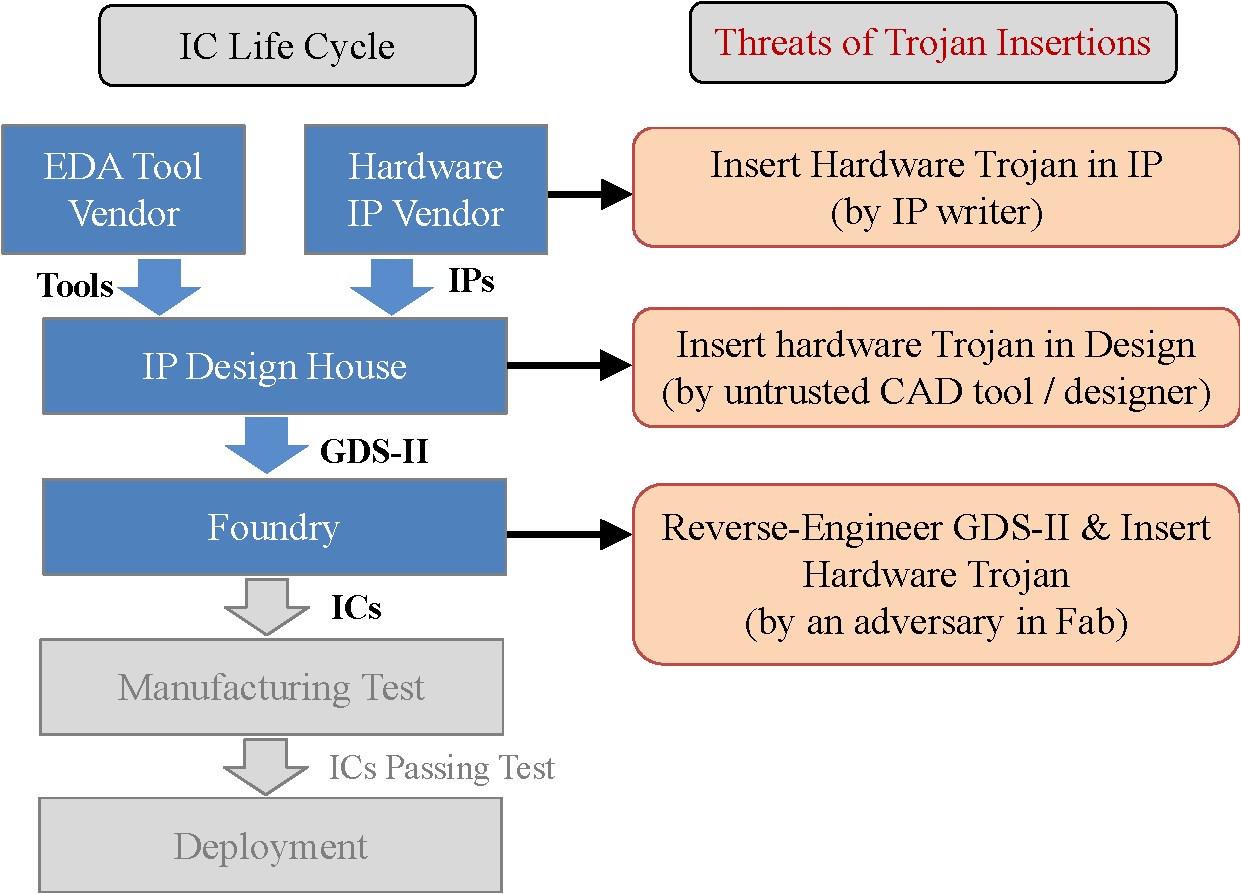
\includegraphics[width=8.5cm]{figure/HT_insert.pdf}
\caption{Hardware Trojan Insertions by different parties at different stages of IC life cycle \cite{article:SB2}.}
\label{fig:assign_result}
\end{figure}

Although hardware Trojans detection methods are implemented in different stages, finding all hardware Trojans cannot be promised even with the most cutting-edge technologies. However, many applications such as banking and military systems have high security requirements, and runtime hardware Trojan detection methodologies attract attention in recent years. Hardware Trojan detection with runtime circuit parameters and runtime verifications are the two most used runtime hardware detection techniques.

\subsection{Hardware Trojan Detection with Runtime Monitoring}

Runtime monitoring detects the hardware Trojans by continuously checking and verifying the behavior of side-channel signals, and recent researchers focused on the improvement of runtime hardware Trojan detection accuracy. He \textit{et al.} \cite{conference:JH} developed a runtime trust evaluation framework based on on-chip EM sensors, and achieved a high detection accuracy of hardware Trojan. Hou \textit{et al.} \cite{article:YH} guarded the concerned signals, and initiated a hardware interrupt request when abnormal toggling events occur. Kulkarni \textit{et al.} \cite{conference:AK}\cite{article:AK} proposed real-time anomaly detection frameworks based on support vector machine and K-nearest neighbor for many core architecture. Zhao \textit{et al.} \cite{article:HZ} proposed a runtime Trojan detection model, which applied chaos theory to characterize side channel parameters in a reconstructed phase space. Malekpour \textit{et al.} \cite{conference:AM} focused on mitigating hardware Trojans with a permanent impact on system and successfully detected the hardware Trojans with a slightly high area and performance overheads.

Researchers also observed the significant increment of resources, power and performance caused by runtime monitoring, and many solutions have been proposed to reduce these increments while maintaining high accuracies of Trojan detection. Mohd \textit{et al.} \cite{article:BM} developed a low-power, low-energy and trusted designed based on a smart runtime monitoring algorithm. Bao \textit{et al.} \cite{article:CB} demonstrated approaches with low hardware resource overheads for runtime Trojan detection with thermal sensors. Zhu \textit{et al.} \cite{article:JZ} obtained a high effectiveness in detecting pervasive hardware security issues, including vulnerabilities and hardware Trojans, with little performance loss. Khalid \textit{et al.} \cite{article:FK} proposed a single power-port current acquisition block using current sensors in time-division multiplexing, which increases detection accuracy with a reduced area overhead. Hussain \textit{et al.} \cite{conference:MH} demonstrated a runtime energy-efficient hardware Trojan localization design for NoCs, where the authentication got activated only when the hardware Trojans were triggered.

The main advantage of SM is the reconfigurability to various checks without the "golden model", but these checks are simple, and do not cover the entire circuit. Therefore, finding all hidden Trojans using SMs still cannot be guaranteed although many researches have been proposed to improve the HT detection efficiency.


%Rajendran \textit{et al.} \cite{article:JR} focused on the ESL design tools and added protection against attacks at the ESL to make it more robust. Guo \textit{et al.} \cite{article:XG} demonstrated an automatic integrated formal verification framework to protect SoC design from the malicious attacks of hardware Trojans.

%Rajendran \textit{et al.} \cite{article:JR} focused on the ESL design tools and added protection against attacks at the ESL to make it more robust

\subsection{Runtime Verification}
Most previous work on HT detection, suggests to source IPs from two different vendors, as it is very unlikely that IPs are infected in the same manner \cite{article:NV}. Therefore, researchers presented design solutions that can detect malicious outputs by duplicating 3PIPs and comparing their results, and they also proposed methods to avoid collusion between parent and child IPs from the same vendor. These design constraints are also named as security constraints, which attempt to detect the triggered hardware Trojans or mute the hardware Trojan attack effects at runtime \cite{article:JR3} \cite{article:SS}, and incorporating security constraints in MPSoC design attracts the attention of recent researchers.

Reecee \textit{et al.} \cite{article:TR} identified hardware Trojans through comparison of two similar untrusted designs, by testing functional differences for all possible input combinations. Beaumont \textit{et al.} \cite{conference:MB} developed an online Trojan detection architecture that implements fragmentation, replication, and voting. Cui \textit{et al.} \cite{conference:XC} implemented both Trojan detection and fast recovery at run-time using re-computation with the IP cores from different vendors, which are essential for mission-critical applications. Rajendren \textit{et al.} \cite{conference:JR2} incorporated security constraints into the higher level design of SoCs and proposed a scheduling method for avoiding malicious output and collusion. Shatta \textit{et al.} \cite{conference:MS} presented methodologies that detect the errors triggered by hardware Trojans in 3PIPs using voter, and recover the system by replacing the error \cite{conference:MS}.

However, fulfilling the security constraints always incurs significant overheads of system performance, chip area and power, which are always sensitive to the designers, and therefore, researchers also started to reduce the resource, performance, and power/energy of MPSoC designs in context of security constraints. Cui \textit{et al.} \cite{article:XC} solves the online HT detection and recovery problem with graph-theoretic models which minimize the implementation cost of design budget and area overhead. Liu \textit{et al.} \cite{article:CL} propose a set of heuristics to ensure that the introduced security constraints creates a minimum impact on the performance and hardware. Wang \textit{et al.} \cite{article:NW} jointly optimized the design budget by reducing the cost of purchasing different IP cores and the system performance, with a minimized security constraint violations. Sun \textit{et al.} \cite{article:YS} minimizes the energy consumption while simultaneously protecting the MPSoC against the effects of hardware Trojans with security constraints.

In summary, these above mentioned works either consider security constraints as hard constraints (constraints that must not be violated) \cite{article:XC} \cite{conference:AS} \cite{article:YS}, which results a very limited optimization space of reducing the system performance, power, and resources; or forgot to minimize the security when optimizing these design targets \cite{article:CL} \cite{article:NW}, leading an extra vulnerability to hardware Trojans. In this work, we jointly optimize the performance and resources of MPSoC while taking account security constraints. Our proposed methods provide solutions that enable designers make tradeoffs between security and system performance, and designer could reduce a significant performance with only a small weakness of security protection.

\section{Problem Description}

In this section, we first demonstrate the motivations of this work which incorporates security constraints in task schedule, and then formulate the problem.
%At present, industry needs to procure and use the latest COTS 3PIPs to track the most cutting-edge technology while reducing the manufacturing costs, but this brings a high risk to the systems.

%\subsection{Threat Model}

%3PIP cores fall into one of the three categories: soft, firm, and hard, depending on their format when they are supplied. \textcolor{blue}{Soft IP cores are described using VHDL or Verilog, and hardware Trojans can be inserted into soft IP cores by IP vendors during IP design}.


%In general, the Register Transfer-Level (RTL) files of IPs might have been imported from third party vendors, and 3PIPs procured from IP vendors are usually not 100\% trustworthy. There may be a rogue insider in a 3PIP house who may insert Trojan logic in 3PIPs coming out of the IP house, and the Trojans may modify function, deny service, or create a backdoor to leak information.% and therefore, hardware Trojan protection strategy during HLS requires attation.



%It is extremely difficult to detect all of the hardware Trojans in 3PIPs since there is no known golden model for 3PIPs. IP vendors usually provide source code, which may contain Trojans. A Trojan can be very well hidden during the normal functional operation of the 3PIP supplied as RTL code. An attacker may distribute few RTL codes so as to reduce Trojan footprint, and a large industrial-strength IP can include thousands of lines of code, resulting in identifying the Trojan in an IP to be an extremely challenging task. When a Trojan exists in an IP, all the fabricated cores will contain Trojans, and detecting all Trojans in an SoC chip is also impossible.



%At present, industry needs to procure and use the latest Commercial-Off-The-Shelf (COTS) electronic components in order to track the most cutting edge technology while reducing the manufacturing costs. However, the hardware Trojans in these COTS components present high risks of malicious inclusions and data leakage in products \cite{conference:XW2}. In the present study, we ignore the threats posed by software Trojans and only consider the protection of applications from hardware Trojans.


%3PIPs procured from IP vendors are not 100\% trustworthy. There may be a rogue insider in a 3PIP house who may insert malicious logic in 3PIPs coming out of the IP house.

%In Trojaned hardware, the attacker may modify the function, deny service, or create a backdoor to leak confidential information, thereby allowing the task running on the malicious intellectual property (IP) core to either generate additional output and trigger Trojans in other IP cores from the same vendor, or to produce incorrect outputs \cite{article:CL}. To protect applications from these risks, most previous studies have either implemented hardware Trojan detection and prevention, or security-aware system level designs.

%Although hardware Trojans detection methods are implemented in different stages, finding all hardware Trojans cannot be promised even with the most cutting-edge technologies. However, many applications such as banking and military systems have high security requirements, and therefore, design-for-security methodologies that mute the hardware Trojan effects require attention.


\begin{figure}[!t]
\centering
\begin{tabular}{cc}
\hspace*{-1.5em}
\subfigure [] {
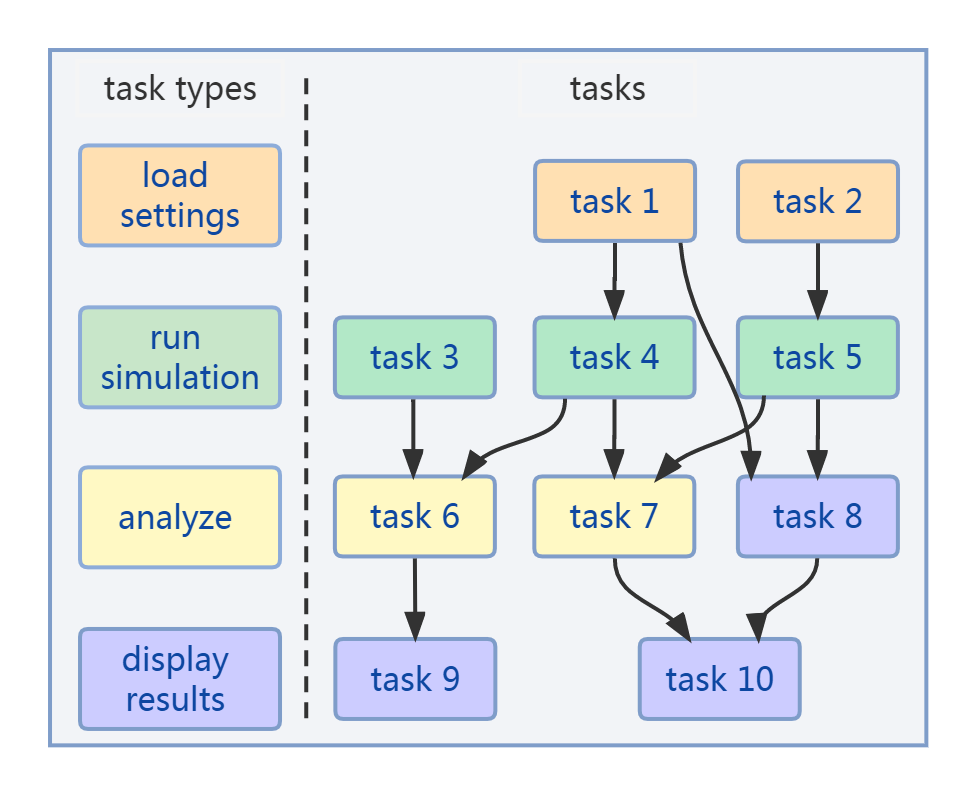
\includegraphics[width=6.0cm]{figure/tg.png}\label{subfig:tg4}
} &\hspace*{-1.5em}
\subfigure [] {
\includegraphics[width=2.6cm]{figure/tg4.pdf}\label{subfig:asap_schedule}
}
\end{tabular}
\begin{tabular}{c}
\subfigure [] {
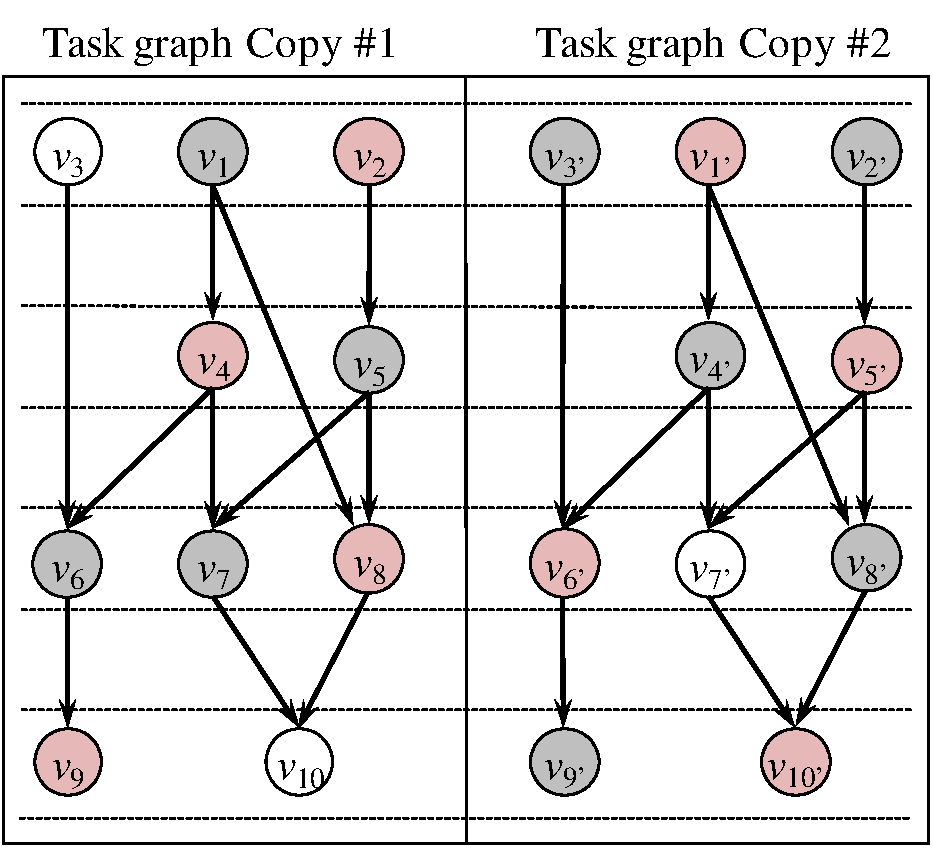
\includegraphics[width=7.2cm]{figure/constraint_example1.pdf}\label{subfig:asap_schedule_security}
}
\end{tabular}
\caption{Example of task graph and its schedules. \subref{subfig:tg4} Task graph. \subref{subfig:asap_schedule} ASAP schedule. \subref{subfig:asap_schedule_security} ASAP schedule with security constraints.}
\label{fig:security}
\end{figure}

\subsection{Security Constraints}
\label{subsect:sec}
The recently proposed security constraints \cite{article:JR3}-\cite{article:NW} enable a trustworthy design using untrusted 3PIPs, and the IPs can be purchased from different vendors without worrying about their individual security problems. All tasks are scheduled and bound to cores under the following two security constraints.%: \textit{task duplication} and \textit{vendor diversity}.


\subsubsection{Task Duplication Constraint}

The probability that the Trojans implanted by different attackers have the same trigger input is quite low, and it is virtually impossible that two cores from different IP vendors will output the same tampered results after the same trigger input. Thus, each task is duplicately executed on the cores from different vendors, and the outputs of these cores will be compared by a trusted component (not designed by the third party) to ensure the trustworthiness of the comparison step \cite{conference:DG}. If the comparison fails, all the dependent tasks are terminated and a security flag is raised.

In the following descriptions, the duplicated task of $v_i$ is denoted as $v_{i'}$.



\subsubsection{Vendor Diversity Constraint}

To mute the Trojan footprint, attackers always distribute Trojans in multiple IP cores and construct secret communications between IP cores to leak information, or to trigger the hibernating Trojans\cite{article:CL}. In this study, we assume that the secret communication between IP cores from the same vendor cannot be acquired by other vendors and that the attackers of different vendors plant different hardware Trojans. Therefore, data-dependent tasks are executed on the cores fabricated from different IP vendors to isolate the triggered hardware Trojans.

%However, the \textit{redundant execution} approaches, including voting architecture \cite{conference:MB}, dual modular redundancy (DMR) \cite{conference:DG}, and task duplication constraint, detect the hardware Trojans by comparing the outputs of cores from different vendors with the same input, and they cannot cut off these secret communications. Thus the vendor diversity constraint which forces the  is also introduced to isolate the triggered hardware Trojans from the rest of the system.

%To mute the Trojan footprint, the attacker always distributes Trojans in multiple IP cores and constructs secret communications between cores to leak information or to trigger the hibernating Trojans. In this study, we assume that the secret communication between cores from the same vendor cannot be acquired by other vendors and that the attackers of different vendors plant different hardware Trojans.

In a task graph with $n$ nodes and $m$ edges, the number of task duplication constraints is $n$, and the number of vendor diversity constraints is $2m$ (both task graph and the duplicated task graph contain $m$ vendor diversity constraints). Therefore, the number of all security constraints (denoted as $scy$) is $n+2m$.

\begin{figure}[!t]
\centering
\begin{tabular}{cc}
\hspace{-1em}
\subfigure [] {
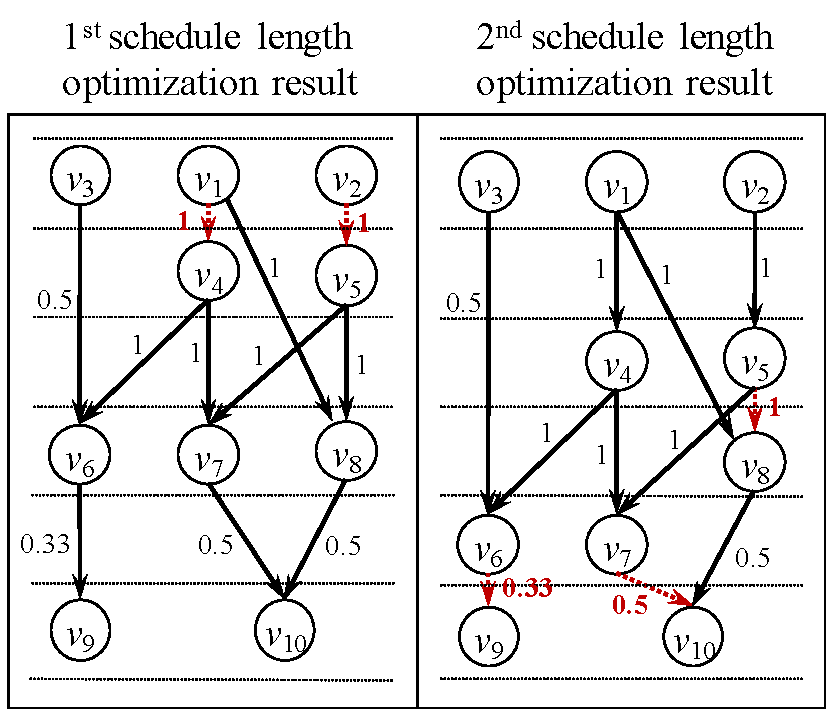
\includegraphics[width=4.4cm]{figure/performance-motivation1.pdf}\label{subfig:performance-motivation1}
} &
\hspace{-1.5em}
\subfigure [] {
\includegraphics[width=4.15cm]{figure/performance-motivation2.pdf}\label{subfig:performance-motivation2}
}
\end{tabular}
\caption{Examples of performance optimization. \subref{subfig:resource_req1} The vendor assignment and its ALAP schedule that totally need 6 cores. \subref{subfig:resource_req2} The vendor assignment and its ALAP schedule that totally need 7 cores.}
\label{fig:resource_req_motivation}
\end{figure}


\subsection{Motivations}
\subsubsection{Security Strength in Performance Optimization}

Fulfills security constraints at the finest granularity, but this incurs significant overhead of system performance. Therefore, researchers also explore the possibility of grouping data-dependent tasks into a cluster and scheduling the entire cluster to a single core to hide the inter-core communication latency \cite{article:CL} \cite{article:NW}. However, Liu \textit{et al.} \cite{article:CL} forgot to minimize the number of violated security constraints, and Wang \textit{et al.} \cite{article:NW} ignored the Trojan attack probability variation to tasks and communications. The reason of must not ignoring Trojan attack probability variation is that attackers always choose critical targets to reduce the Trojan footprint while creating large damage to the system, resulting different attack probabilities to tasks and communications.




The example in Fig. \ref{fig:security} demonstrates the above reason, and in the following paper, clustering the connected nodes into one cluster is denoted as \textbf{edge contraction}, and the edge that connects two clustered nodes is called \textbf{contracted edge}. In this example, 10 tasks are sorted into 5 different types (see Fig. \ref{subfig:tg4}), and the computational times of all tasks are assumed to be 1 unit of time (\textit{u.t.}), which also equal their inter-core communication delays. Fig. \ref{subfig:asap_schedule} shows the as-soon-as-possible (ASAP) schedule, and the optimization target is to reduce schedule length by 1 \textit{u.t.}. Traditional methods \cite{article:NW} contract the least number of edges, and $e_{1,4}$ and $e_{2,5}$ will be contracted. However, attackers may likely to modify the system settings to crash the whole system or output their desired results, meaning that edges $e_{1,4}$ and $e_{2,5}$ require a high priority protection. In stead, tasks 8-10 save the settings and demonstrate the final results, and probabilities of attacking these tasks and related communications are much lower. Therefore, contracting $e_{6,9}$, $e_{7,10}$ and $e_{8,10}$ causes less Trojan attack risks to the system, even though this violates a larger number of security constraints.


%For example, some tasks may gather the systems status, and some tasks are responsible for calculation whose results may contain critical information, and so on. Therefore, the possibility of attack lay to each task will also be different. To better protect our systems for hardware Trojan while some of the security constraint 2 must be removed due to the schedule length optimization, each communication should be assign with an identical priority of protection. In the example shown in Fig. \ref{subfig:security2} where the target is to optimize the schedule length by 10 $u.t.$, clustering $v_5$ and $v_6$, $v'_5$ and $v'_6$ violates the less number of security constraint violations. However, $v_5$ may output important information that must be protected, and thus, we should consider other task clustering solutions other than clustering $v_5$ and $v_6$.
%The scheduling effects to the number of cores required and the amount of data fetched from off-chip memory are illustrated in Fig. \ref{fig:TG2}, where the performance constraint is set to 70$ms$, and we assume that each core need 1$ms$ to execute a task with 1 ($u.t.$), and the inter-core communication delay equals the computational delay. The computational cost and the mobility of each task are denoted beside the task, and the inter-core communication delay is also denoted next to the edge with red color. The scheduling result in Fig. \ref{subfig:TG2-2} requires four cores to execute all tasks, and these tasks totally need to fetch 55 ($u.m.$) data from off-chip memory. Regarding the scheduling result in Fig. \ref{subfig:TG2-3}, two cores are required, and only 40 ($u.m.$) data are fetched from the off-chip memory because $v_2$ and $v_3$ shares 10 ($u.m.$) common input data and $v_4$ and $v_5$ shares 5 ($u.m.$) common input data. These data can be temporarily stored in SPMs and later used by the other tasks if these tasks are assigned to the same core.% thus, $v_4$ no longer needs to fetch the input data from the off-chip memory.
%\begin{figure}[!ht]
%\centering
%\begin{tabular}{ccc}
%\hspace{-1.6em}
%\subfigure [] {
%\includegraphics[width=4.2cm]{figure/TG2.pdf}\label{subfig:TG2-1}
%}  &\hspace{-1.6em}
%\subfigure [] {
%\includegraphics[width=1.85cm]{figure/TG2-2.pdf}\label{subfig:TG2-2}
%} &\hspace{-0.5em}
%\subfigure [] {
%\includegraphics[width=1.85cm]{figure/TG2-3.pdf}\label{subfig:TG2-3}
%}
%\end{tabular}
%\caption{Example that shows the effects on the number of cores required and the visits to the off-chip memory due to different scheduling results. \subref{subfig:TG2-1} Example of $TG$. \subref{subfig:TG2-2} The 1st scheduling result. \subref{subfig:TG2-3} The 2nd scheduling result.}
%\label{fig:TG2}
%\end{figure}



\begin{figure}[!t]
\centering
\begin{tabular}{c}
%\hspace{-1em}
\subfigure [] {
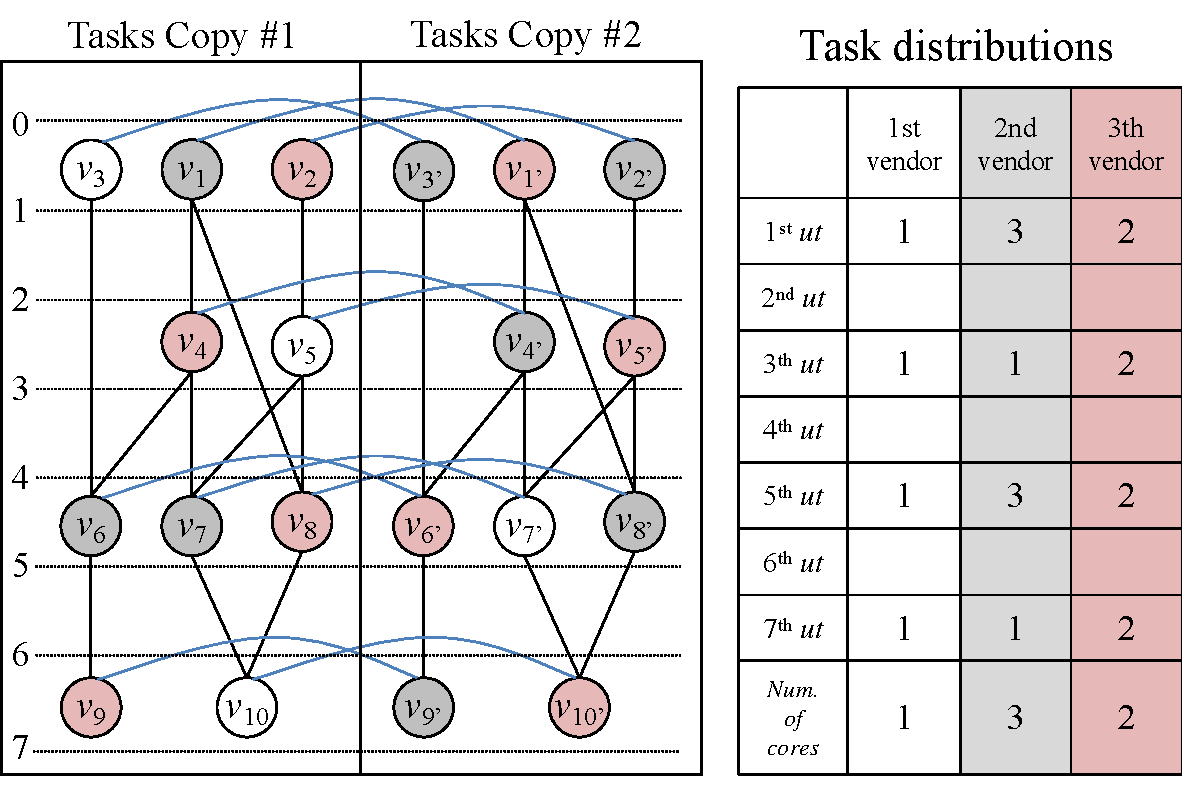
\includegraphics[width=8.4cm]{figure/security1.pdf}\label{subfig:resource_req1}
} \\
%\hspace{-1em}
\subfigure [] {
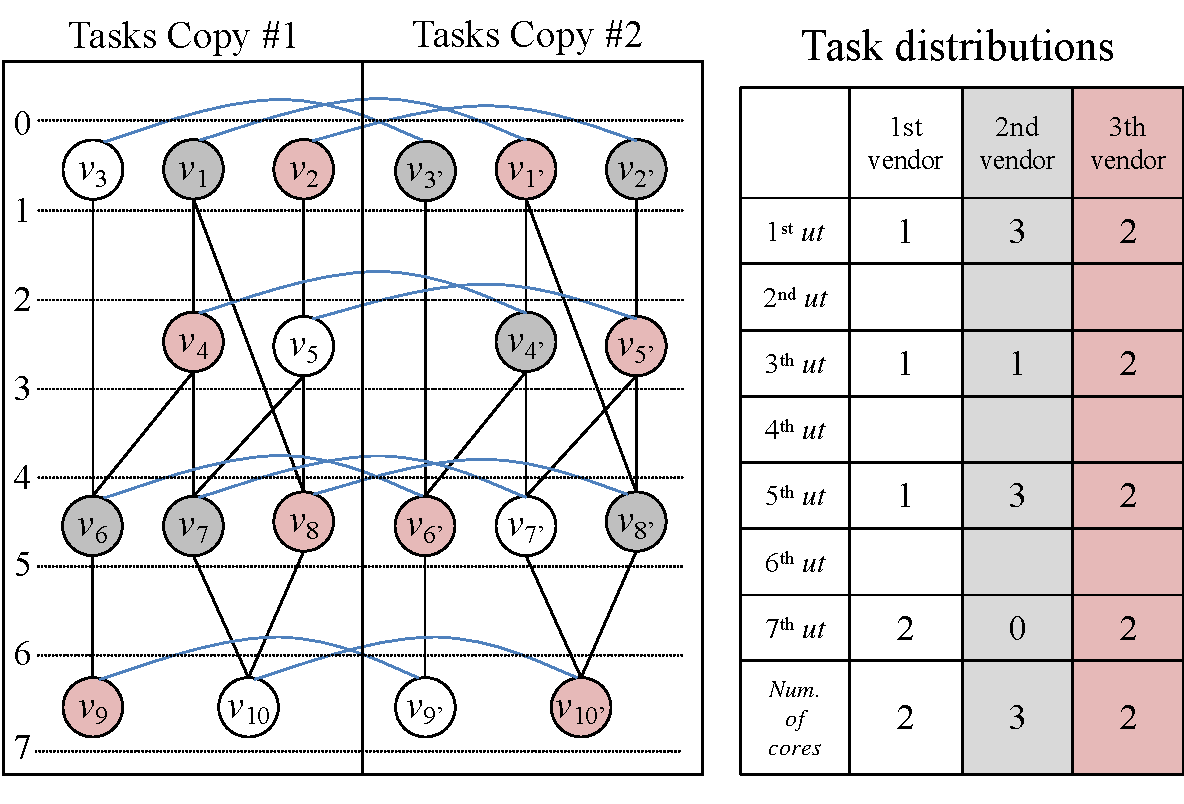
\includegraphics[width=8.4cm]{figure/security2.pdf}\label{subfig:resource_req2}
}
\end{tabular}
\caption{Example of resource optimization in vendor assignment. \subref{subfig:resource_req1} The vendor assignment and its ASAP schedule who totally needs 6 cores. \subref{subfig:resource_req2} The vendor assignment and its ASAP schedule who totally needs 7 cores.}
\label{fig:resource_req_motivation}
\end{figure}

\subsubsection{Resource Optimization in Vender Assignment}

Satisfying security constraints incurs a significant increment of hardware resources, including the number of cores integrated in the SoC. Although we assume that security is the top target when designing circuits, the area of circuit must not be neglected. Traditional methods \cite{article:CL} \cite{article:NW} only minimized the core usages in task scheduling, and the number of cores can be further optimized if we start to consider core reduction during vendor assignment.


The example in Fig. \ref{fig:resource_req_motivation} illustrates the necessity of optimizing the core usages during vender assignment. In this example, tasks colored white, gray, and pink are assigned to 1st vendor, 2nd vendor, and 3rd vendor, respectively. $v_{i'}$ is the duplicate of $v_i$, and the lines between tasks are colored blue and black, which represent the \textit{task duplication} and \textit{vendor diversity} constraints, respectively. The performance constraint is assumed to be 7 $u.t.$, and the computational time of each task and the inter-core communication delay are both 1 $u.t.$. Fig. \ref{subfig:resource_req1} and Fig. \ref{subfig:resource_req2} give two different vendor assignment results, and their tasks are all scheduled by as-late-as-possible (ALAP) method. With the vendor assignment given in Fig. \ref{subfig:resource_req1}, the scheduling results require 6 cores, but 7 cores are required with the vendor assignment shown in Fig. \ref{subfig:resource_req2}.

\subsection{Problem Formulation}

Let the task graph be $TG=(V,E)$, where $V$ is the set of all tasks and $E$ represents the data dependencies between tasks. The optimization problem we focused in this study is named as the security-aware task scheduling problem with performance and area optimization. The performance optimization target is set as the constraint that the schedule length must not exceed, and the area is optimized by reducing the number of cores integrated in the SoC. In this paper, we assume that Trojans cannot successfully attack the protected tasks and communications, while the unprotected ones have different possibilities of being attacked.

\begin{problem}
Inputs: task graph $TG$, performance constraint, and security constraints. The target is to find a schedule with a least system risk, and the number of cores required is also minimized.
\end{problem}

The objective function of the above problem is formulated as follows.
\begin{equation}
min:~\alpha*risk_s+core
\end{equation}
\noindent where $risk_s$ is the system risk, $core$ is the number of cores required by the schedule, and $\alpha$ is a parameter large enough to keep the minimization of system risk as the first priority.

Schedule length optimization violates the vendor diversity constraints, and only communications may be successfully attacked by the triggered hardware Trojans. Let $risk(e)$ be the probability that $e$ is a communication attack target, and $E_c$ be the set of contracted edges in both $TG$ and $TG'$. The system risk $risk_s$ caused by hardware Trojans can be calculated as follows.
\begin{equation}
risk_s=1-\prod \limits_{e\in E_c}(1-risk(e))
\end{equation}


In this work, the calculation of $risk(e)$ is decided by system designers. All possible reasons of the Trojan attack via $e$ should be considered, such as the types of connected tasks, the importance of information transmitted, and the difficulty of leaking information.

%To simplify the experiments, the core speeds of all vendors are assumed to be the same. If the core speeds of different vendors vary, this proposed method can easily be extended to fit.

%\begin{definition}[\textit{\textbf{Execution interval}}]
%The \emph{execution interval} ($EI$) of $v_i$ is defined as a consecutive time period with a length of $exec(v_i)$, where $exec(v_i)$ is the acutual execution time of $v_i$; it is denoted as $EI^{v_i}_{st}$ if its starting time is $st$. After scheduling, we write $EI^{v_i}=[s(v_i), f(v_i)]$ for simplicity.% where $s(v_i)$ and $f(v_i)$ are the starting and finishing times, respectively, of executing $v_i$.
%\end{definition}




%After assigning each task to a appropriate vendor, the real execution times of tasks can be determined, and the schedule length is calculated, which may violate the input performance constraint because we assumed that all the tasks are executed with the fastest core-speed during the task clustering stage. Let $p_c$ be the input performance constraint, $p_c'$ be the virtual performance constraint used in the task clustering stage which is initialized as $p_c$, and $sl$ be the schedule length. The principal of performing performance-constrained vendor assignment is to iteratively shorten the $p_c'$ by the schedule length overhead ($sl-p_c$) and then to execute the task clustering and vendor assignment until $sl \leq p_c$. This process is described by the pseudo codes in Algorithm \ref{alg:task_scheduling} (\textit{Lines} 2-12).

%\subsection{Performance-Constrained Task Scheduling}

%The scheduling result decides the number of cores integrated in a MPSoC and also brings significant effects to the amount of data fetched from the off-chip memory. In this work, the unit of memory ($u.m.$) is used to describe the amount of data.% Scheduling tasks evenly in each time period helps reduce the number of required cores, while maximizing the sharing of common input values in SPMs significantly reduces the amount of values fetched from the off-chip memory.

%An example of mobility derived from Fig. \ref{subfig:TG2-1} is given in Fig. \ref{subfig:mobility1}, where the computational cost of each task and the inter-core communication delay are both 10 ($u.t.$).




\section{Security-Aware Task Scheduling with Performance and Area Optimization}

In this section, our proposed task scheduling method is presented in details. The system performance is first optimized along with the Trojan attack risk, and tasks are then assigned to IP vendors and scheduled to time periods with core usage optimization.% that can share the same core are assigned to the same IP vendor and scheduled by force-directed scheduling method to minimize the  number of cores.% assigned to IP vendora task cluster-based vendor assignment method assigns tasks that can share the same core to the same IP vendor; finally, a force-directed method is used to schedule all tasks with a minimized number of cores.

\subsection{Performance-Constrained Task Clustering}
System performance is one of the key considerations for designers, and they always put several timing-critical tasks into the same core to minimize the schedule length \cite{article:CL} \cite{article:NW}. However, this brings potential Trojan attack risk to the system, which must not be neglected in performance optimization.% In this section, several edges are contracted to satisfy the performance constraint; meanwhile, the number of contracted edges and the amount of data stored in the off-chip memory are simultaneously optimized.

\begin{figure}[!t]
\centering
\begin{tabular}{ccc}
\hspace*{-1em}
\subfigure [] {
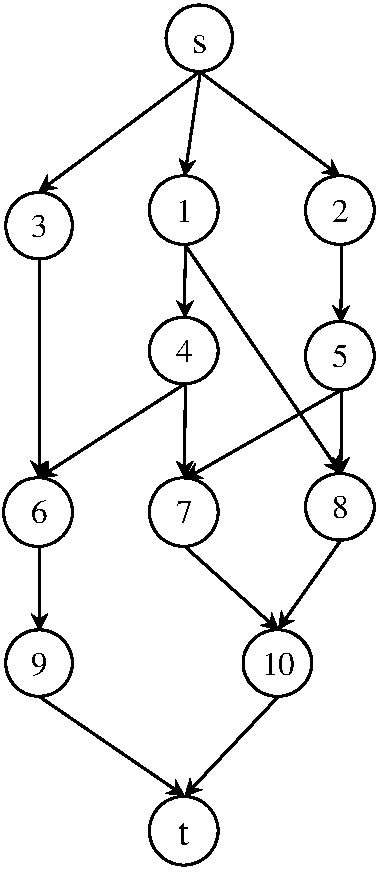
\includegraphics[width=2.3cm]{figure/TG1.pdf}\label{subfig:TG1}
}&\hspace*{-1.6em}
\subfigure [] {
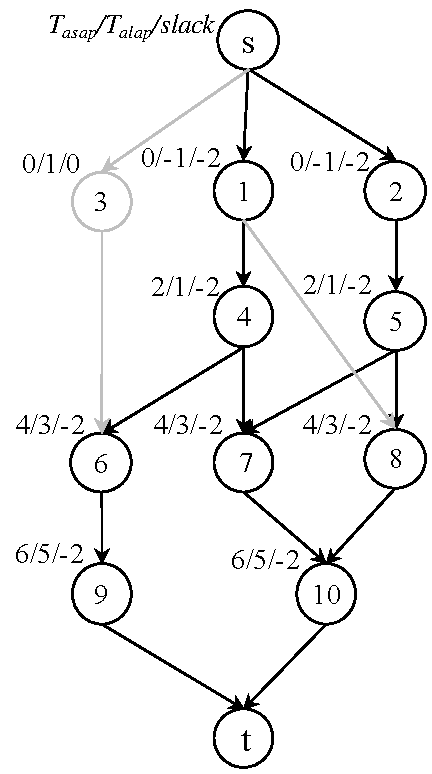
\includegraphics[width=3cm]{figure/tvg.pdf}\label{subfig:tvg1-1}
} &\hspace*{-1.6em}
\subfigure [] {
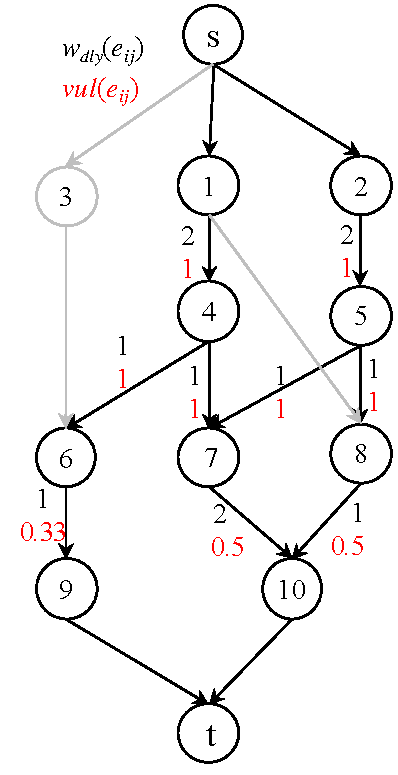
\includegraphics[width=3.05cm]{figure/tvg1.pdf}\label{subfig:tvg1-2}
}
\end{tabular}
\caption{Example of evaluating timing violated graph. \subref{subfig:TG1} Task graph with $s$ and $t$. \subref{subfig:tvg1-1} $TVG$ with timing constraint to be 5 $u.t.$ \subref{subfig:tvg1-2} The evaluation of $w_{dly}(e)$.}
\label{fig:weight_e}
\end{figure}

We only discuss the method of contracting edges in $TG$ in the following description, and schedule length optimization of $TG'$ can be performed in the same manner. Let $slack(v)$ be the slack time of $v$ under the performance constraint, and it is calculated as follows.
\begin{equation}
slack(v) = t_{alap}(v)-t_{asap}(v)-exec(v)
\end{equation}

\noindent where $exec(v)$ is the execution time of task $v$, and $t_{asap}(v)$ and $t_{alap}(v)$ are the ASAP and ALAP schedules, respectively.% Fig. \ref{subfig:TG2} gives an example of calculating the slack time of each task in $TG$, where the virtual execution time of each task and the inter-core communication delay are both 1 ($u.t.$), and the virtual performance constraint is 5 $(u.t.)$.% The ASAP scheduling and ALAP scheduling results, and the slack times of tasks are denoted next to the tasks.% Then, the schedule length of $TG$ is iteratively reduced by contracting edges until this $TVG$ is empty.

Source and sink nodes $s$, $t$ are added to $TG$, and directed edges that pointing from $s$ to 0-indegree nodes, and from 0-outdegree nodes to $t$, are also added. An example of task graph with $s$ and $t$ is given in Fig. \ref{subfig:TG1}. \textbf{Timing violated graph} ($TVG=(V_T, E_T)$) is then constructed, and it is an induced subgraph of $TG$. $V_T$ consists of $s$, $t$ and all tasks with negative slacks, and $E_T=\{(v_i,v_j)\in E, v_i\in V_T \textrm{~and~} v_j\in V_T\}$. Let $dly(e_{ij})$ be the inter-core communication delay of $e_{ij}$, and all intra-core communication delays are ignored in this work. Fig. \ref{subfig:tvg1-1} gives an example of $TVG$, where the performance constraint is 5 $u.t.$ and $dly(e)$ is 1 $u.t.$ for each edge.


Data-dependent tasks will be assigned to the same core to reduce the system performance by changing the inter-core communication delay to a much smaller intra-core communication delay. These intra-core communications are denoted by contracted edges in graphs, and sets of edges in $TVG$ will be contracted until the performance constraint is satisfied.% Regarding the tasks: 1) consuming the same data, or 2) feeding their computed data to the same task, they must not be assigned to the same core.




Contracting an edge ($e_{ij}$) with $k(u.t.)$ reduces the lengths of all paths that passing though $e_{ij}$ by $k(u.t.)$. Let $w_{dly}(e_{ij})$ be the sum of the reduced schedule lengths of all paths (from $s$ to $t$) in $TVG$ after contracting $e_{ij}$, and it is calculated by the following equation.
\begin{equation}
w_{dly}(e_{ij})=path_{tvg}(e_{ij})*dly(e_{ij})
\end{equation}


\noindent where $path_{tvg}(e_{ij})$ is the number of paths in $TVG$ that pass through $e_{ij}$.

Fig. \ref{subfig:tvg1-2} illustrates the $w_{dly}(e)$ in $TVG$, which are indicated next to the edges. The $dly(e)$ of all edges are 1, making $w_{dly}(e)$ equals $path_{tvg}(e)$ in this example. Choosing the edges with larger $w_{dly}(e_{ij})$ indicates that less edges will be contracted until the performance constraint is reached.



%\noindent where $risk(e_{ij})$ is the evaluated possibility that Trojan attacks through this communication. and $path_{tvg}$ is the number of all paths in $TVG$. Fig. \ref{subfig:tvg1-2} illustrates the $w_{dly}$ in $TVG$, which is indicated next to the edge.





%Clustering of timing critical tasks also necessitates information of task criticality.
The total weight that evaluates an edge $e_{ij}$ contraction in $TVG$ is denoted as $w(e_{ij})$, which is calculated as follows.
\begin{equation}
w(e_{ij}) = \frac{w_{dly}(e_{ij})}{risk(e_{ij})}
\label{equ:weight_e}
\end{equation}

\noindent where $risk(e_{ij})$ denotes the probability that Trojan may attack the system via edge $e_{ij}$.

However, not all edges can be contracted with respect to the multi-core parallel execution. Let $in\_edge(v)$ be the set of edges that end with $v$, and $out\_edge(v)$ be the set of edges that start from $v$. Edges in $TG$ that belong to the same $in\_edge(v)$ or $out\_edge(v)$ are called \textbf{brother edges}. If an edge is contracted during performance optimization, all its brother edges can no longer be contracted. The reason is that contracting brother edges makes the tasks that once can be executed parallel in different cores, now must be executed sequentially in the same core, and this may result an increased schedule length. For example, contracting the brother edges $e_{4,6}$ and $e_{4,7}$ in Fig. \ref{subfig:tvg1-2} makes $v_6$ and $v_7$ must be conducted sequentially in the same core, but they once can be computed at the same time in different cores.




Then, a weighted \textbf{edge contraction conflict graph} ($ECCG=(V_E,E_E)$) is constructed to represent if every pair of edges can be contracted simultaneously. Each vertex in $V_E$ represents an edge in $TVG$ that can be contracted, and the weight of a vertex in $V_E$ equals the weight of the corresponding edge in $TVG$. Two vertexes in $V_E$ are connected when their corresponding edges cannot be contracted simultaneously, under one of the following two situations.

\begin{enumerate}
\item These two edges are brother edges (respect to the multi-core parallel execution);
\item These two edges belong to the same path in $TVG$ (for each path in $TVG$, only one edge can be contracted in each iteration, such that the path length will not be over optimized).
\end{enumerate}


\begin{figure}[!t]
\centering
\begin{tabular}{ccc}
\hspace*{-1.0em}
\subfigure [] {
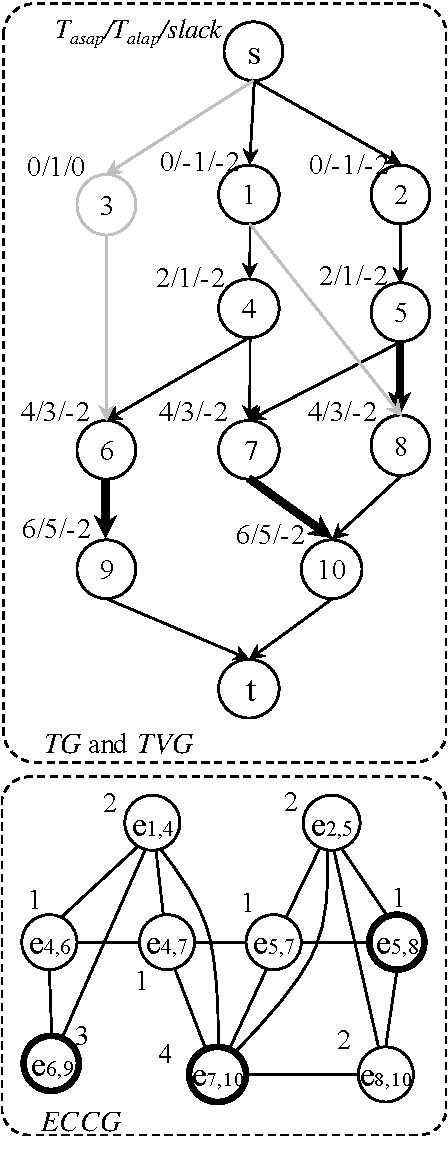
\includegraphics[width=2.8cm]{figure/EVG1.pdf}\label{subfig:EVG1}
} &\hspace*{-1.7em}
\subfigure [] {
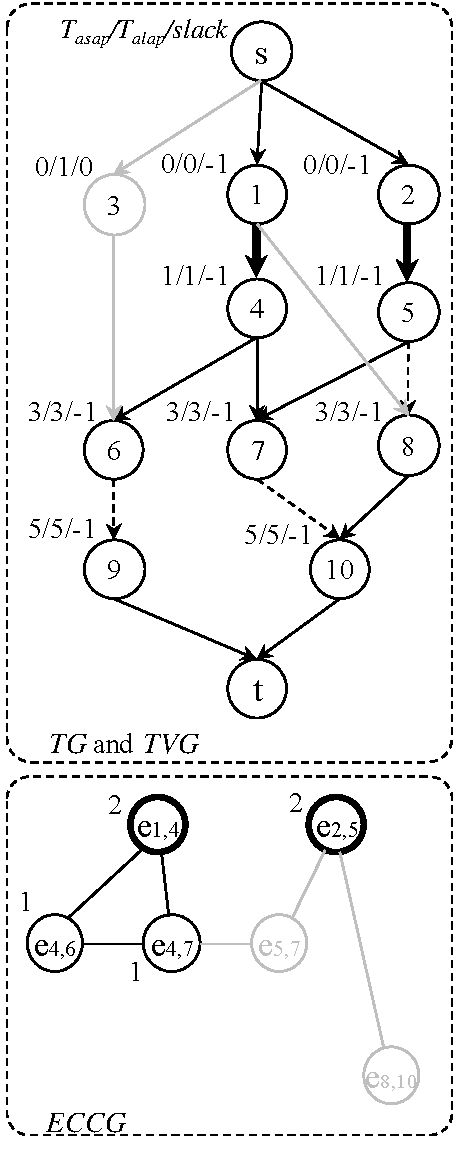
\includegraphics[width=2.8cm]{figure/EVG2.pdf}\label{subfig:EVG2}
} &\hspace*{-1.7em}
\subfigure [] {
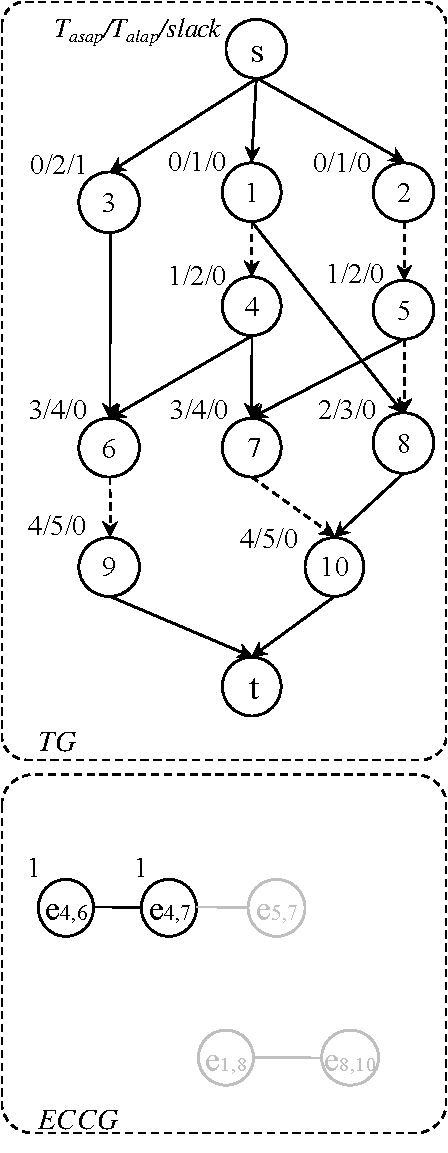
\includegraphics[width=2.8cm]{figure/EVG3.pdf}\label{subfig:EVG3}
}
\end{tabular}
\caption{Example of performance-constrained task clustering procedure. \subref{subfig:EVG1} The $TVG$ and its corresponding $ECCG$ before task clustering. \subref{subfig:EVG2} The $TVG$ and its corresponding $ECCG$ after the 1st iteration of task clustering. \subref{subfig:EVG3} The $TVG$ and the corresponding $VCG$ after the 2nd iteration of task clustering.}
\label{fig:TC}
\end{figure}


%Contracting edges may increase the number of IP vendors required, and if contracting an edge violate the IP vendor constraints (the method in \cite{article:NW} is applied to calculate the number IP vendors), such edge will be removed from $ECCG$.

The maximum weight independent set (MWIS) of the weighted $ECCG$ is calculated by the method proposed in \cite{conference:LC}, and the set of edges in MWIS will be contracted with the maximum benefits among all possible optimization results. Algorithm \ref{alg:PCTC} gives the details of performance-constrained task clustering algorithm with the target of minimizing the Trojan attack risk. In the first step (\textit{lines: 2-5}), $TVG$ is constructed from $TG$, and the weights of all edges in $TVG$ are evaluated. In the second step (\textit{lines: 6-10}), the weighted $ECCG$ is built, and its MWIS is calculated. In the third step (\textit{lines: 11-13}), the MWIS-selected edges in $TG$ are contracted. These three steps are iteratively repeated until the performance constraint is met.

\begin{algorithm}[!h]
\caption{Task clustering with performance constraint, $task\_cluster(TG, pc)$.}
\label{alg:PCTC}
\begin{flushleft}
{Input:}
task graph, $TG$;\\
\hspace*{2.8em}performance constraint, $pc$.\\
{Output:} performance-constrained clustering result, $TC$.
\end{flushleft}
\begin{algorithmic}[1]
\WHILE{$TG.schedule\_length > pc$}
\STATE Construct $TVG$ from $TG$.
\FOR{each $e$ in $TVG$}
\STATE Calculate $w(e)$;
\ENDFOR
\STATE Construct $ECCG$ from $TVG$;
\FOR{Each node $e$ in $ECCG$}
\STATE $ECCG.node\_weight(e)=w(e)$;
\ENDFOR
\STATE Calculate $MWIS$ in $ECCG$;
\FOR{each node $e$ in $MWIS$}
    \STATE Contract the corresponding edge $e$ in $TG$;
\ENDFOR
\ENDWHILE
\end{algorithmic}
\end{algorithm}




With the probabilities of communication attack given in Fig. \ref{subfig:tvg1-2}, an example of performance-constrained task clustering procedure is presented in Fig. \ref{fig:TC}, where we are about to optimize the schedule length by 2 $u.t.$. The $TVG$ consists of the nodes and edges with black color, and dashed lines are the contracted edges. The $ECCG$ is given beneath the corresponding $TVG$, and the weight of contracting an edge is marked next to the node in $ECCG$. The $TVG$ and its corresponding $ECCG$ are first constructed (see Fig. \ref{subfig:EVG1}), and its MWIS is $\{e_{5,8}, e_{6,9}, e_{7,10}\}$ which will be contracted in the first iteration. Then, $TVG$ is updated and $ECCG$ is re-constructed as shown in Fig. \ref{subfig:EVG2}, where $e_{5,7}$ and $e_{8,10}$ are not in $ECCG$ because their brother edges $e_{5,8}$ and $e_{7,10}$ are already contracted. The MWIS of current $ECCG$ is $\{e_{1,4}, e_{2,5}\}$, and after contracting these edges, Fig. \ref{subfig:EVG3} gives the final clustering results, with performance constraint satisfied.% and the corresponding $ECCG$, and $e_{5,8}$ is contracted in the final iteration.



\subsection{Vendor Assignment with Core Minimization}

With performance-constrained task clustering results, we will assign tasks to IP vendors and schedule tasks from the same IP vendor together. The principle of vendor assignment is to iteratively cluster tasks into a number of $v_c$ (vendor constraint) clusters, and assign each cluster with an IP vendor. Different from the task clustering in performance-constrained task clustering stage that violates the vendor diversity constraints by clustering date-dependent tasks, clustering (also named as \textbf{cluster merging}) in vendor assignment follows all security constraints.%, and only clusters tasks that can be assigned with the same IP vendor. % The speed variations of cores between different IP vendors are neglected in this paper.

\textbf{Vendor conflict graph} ($VCFG=(V_c, E_{cf})$) is constructed from the performance-constrained clustering result, where $V_c$ is the set of all clusters from $TG$ and $TG'$. A cluster is determined by the following two situations: 1) a task that is not connected by any contracted edge is regarded as a cluster; 2) tasks that are connected to each other by contracted edges are in the same cluster, and the index of this cluster is decided by the minimum index of the tasks in this cluster. $E_{cf}$ is the set of all edges in $VCFG$, representing that the connected clusters cannot be assigned to the same IP vendor. If two tasks must be assigned to different IP vendors due to the security constraints, the two clusters that contain these two tasks will be connected in $VCFG$.

\textbf{Vendor compatible graph} ($VCPG=(V_c, E_{cp})$) is the complement graph of $VCFG$, and an edge in $E_{cp}$ indicates that the connected clusters can be assigned to the same vendor. Fig. \ref{subfig:vcg_c_1} gives the examples of $VCFG$ and $VCPG$, which are constructed from the performance-constrained clustering results showed in Fig. \ref{subfig:EVG3}. Since the edges in $VCPG$ are too many to demonstrate all, we use dash lines to represent the rest edges connected to this cluster.

%The principle of vendor assignment is to iteratively cluster tasks into a number of $v_c$ (vendor constraint) clusters, and then assign each cluster with a IP vendor.



\begin{figure}[!t]
\centering
\begin{tabular}{c}
\hspace*{-0.5em}
\subfigure [] {
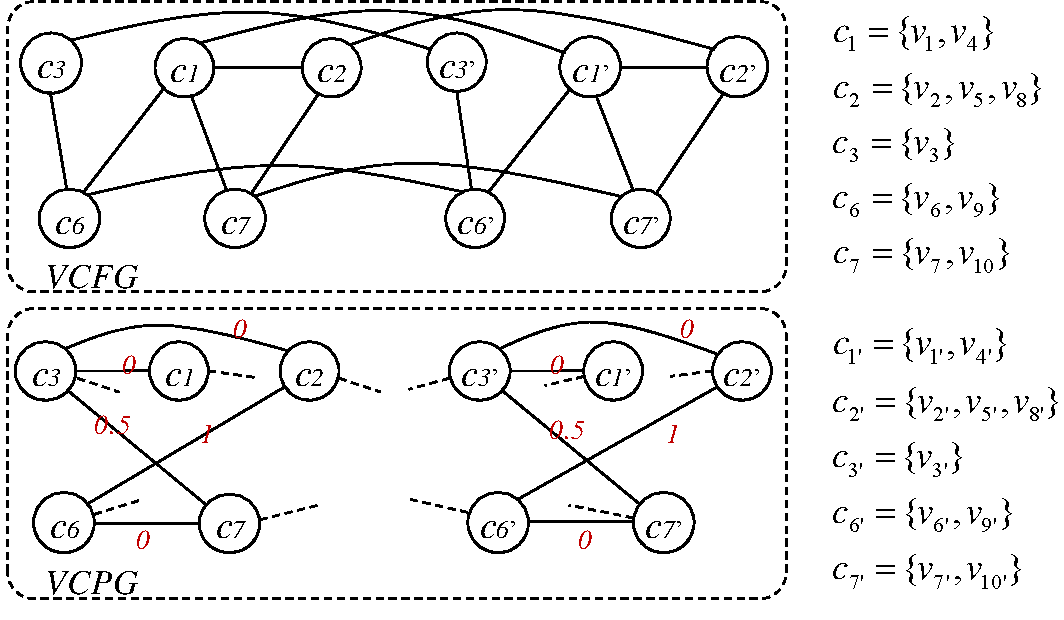
\includegraphics[width=8.6cm]{figure/vcg_c_1.pdf}\label{subfig:vcg_c_1}
}\\\hspace*{-1.2em}
\subfigure [] {
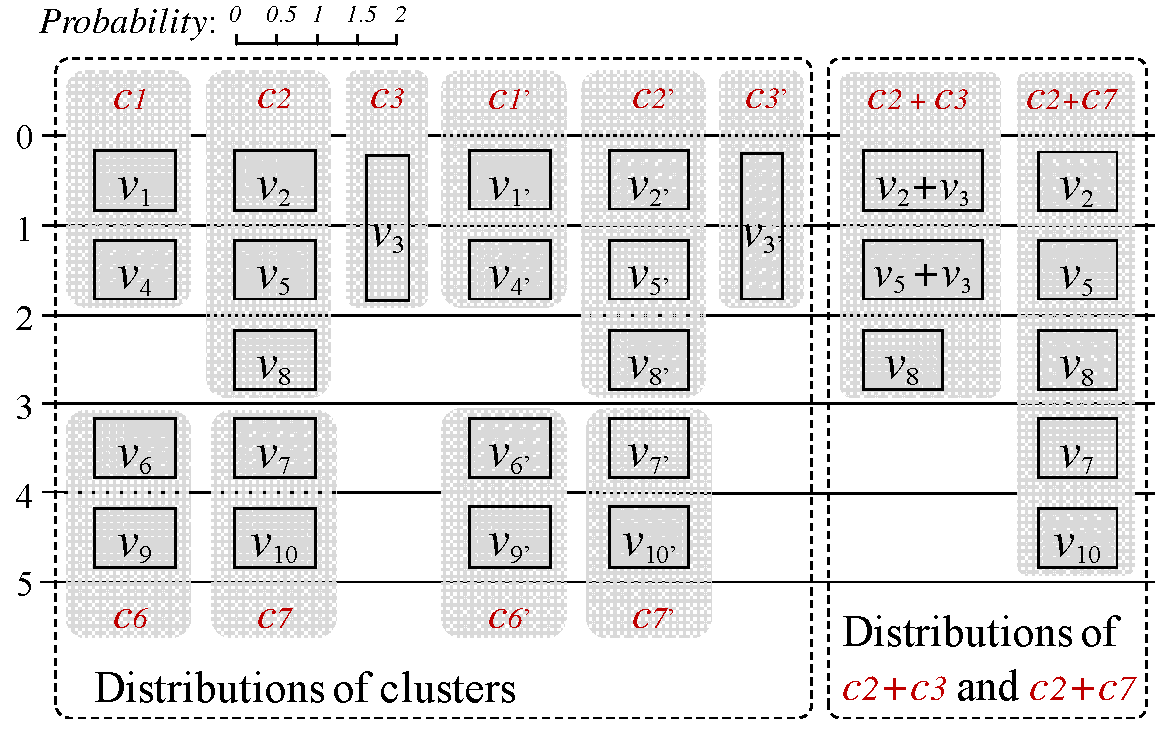
\includegraphics[width=8.8cm]{figure/vcg_c_2.pdf}\label{subfig:vcg_c_2}
}
\end{tabular}
\caption{Example of evaluating vendor compatible graph. \subref{subfig:vcg_c_1} $VCFG$ and $VCPG$ derived from the task clustering results. \subref{subfig:vcg_c_2} Distributions of clusters.}
\label{fig:vc_c}
\end{figure}




%\textit{\textbf{candidate vendor set}} of $c_i$ comprises all of the IP vendors that can be assigned to cluster $c_i$, which is denoted as $cvs(c_i)$. For an edge $e_{ij}$ that connecting $c_i$ and $c_j$, it cannot be contracted if $cvs(c_i)\cap cvs(c_j)=\emptyset$.

%The $c_i$ that can be assigned with $ipv_k$ only when

%\begin{enumerate}
%\item $\forall c_j \in VCG.adj\_node(c_i)$, $cvs(c_j)-ipv_k \neq \emptyset$;
%\item If $v_i$ is assigned with $ipv_k$, the clique size of the new $VCG$ will not violate the vendor constraint.
%\end{enumerate}


%\begin{figure}[!t]
%\centering
%\begin{tabular}{c}
%\subfigure [] {
%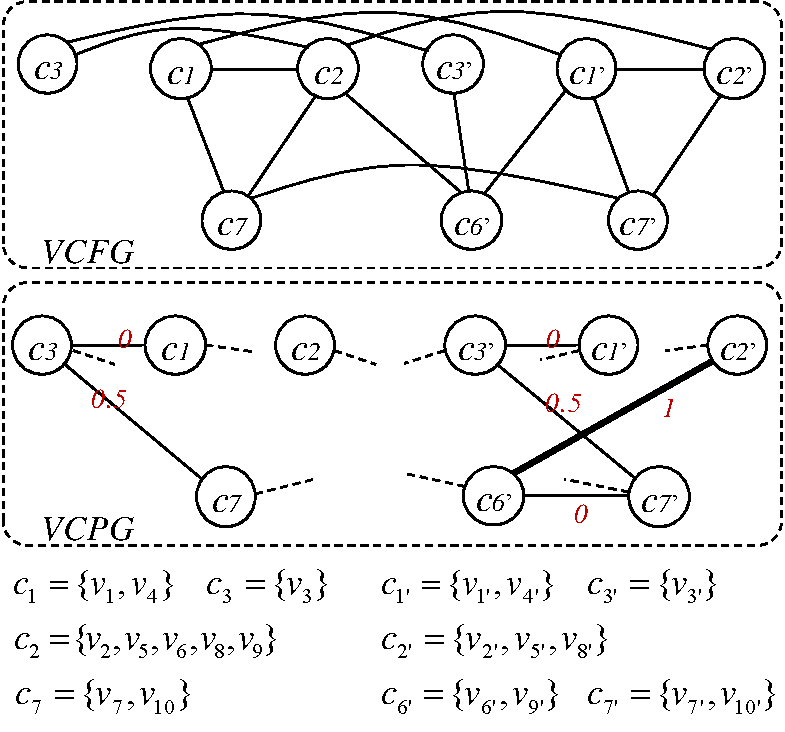
\includegraphics[width=6.3cm]{figure/vcg1.pdf}\label{subfig:vcg1}
%} \\
%\subfigure [] {
%\includegraphics[width=8cm]{figure/dg1.pdf}\label{subfig:assign1}
%}
%\end{tabular}
%\caption{Example of candidate vendor set. \subref{subfig:vcg1} Vendor conflict graph. \subref{subfig:assign1} The candidate vendor set of each cluster.}
%\label{fig:resource_req}
%\end{figure}

%At the very beginning of vendor assignment, each cluster can be assigned with all IP vendors. Each time we update the $vcs$ of a task, all $vcs$ of adjacent tasks will be updated. Fig. \ref{subfig:vcg1} gives the $VCG$ derived from both $TG$ and $TG'$, at the assumption that $v_3$ and $v_6$ are assumed to be assigned to $ipv_1$ and $ipv_3$, respectively; The candidate vendor set of each task is presented in Fig. \ref{subfig:assign1}.

Then, the accumulated probability of task concurrency is introduced to estimate the number of cores required during vendor assignment. The \textbf{mobility} of a task $v_{i}$ is denoted as $M(v_i)$ and defined as a set of consecutive time periods $M(v_{i})=[t_{asap}(v_{i}),~t_{alap}(v_{i})]$.% where $t_{asap}(v_i)$ and $t_{alap}(v_i)$ are the ASAP scheduling and ALAP scheduling results, respectively.% Then, the \textit{mobilities} of all tasks are calculated and the \textit{distribution graph} \cite{article:PP} for each cluster is constructed to estimate the number of cores required during vendor assignment.

Let $prob(v_i,t_j)$ be the probability that $v_i$ is executed in time $t_j$, and the summation of the probabilities of all tasks in a cluster $c$ for the time period $t_j$ is named as the \textit{distribution graph} (DG) \cite{article:PP}, which also indicates the concurrency of tasks. The distribution graph of cluster $c$ in time period $t_j$ is denoted as $DG(c, t_j)$ and calculated as follows.
\begin{equation}
DG(c, t_j) = \sum \limits_{v_i\in c} prob(v_i, t_j)
\end{equation}


The maximum of all $DG(c, t_j), ~\forall t_j\in[1, p_c]$ is denoted as $DG_{max}(c)$, which is used to estimate the number of cores required for all tasks in cluster $c$. Fig. \ref{subfig:vcg_c_2} presents the distribution graphs of all clusters, where the width of a task means the probability that this task will be conducted at the corresponding time period. The reduction of cores required by merging two cluster $c_i$ and $c_j$ is denoted as $Merge(c_i, c_j)$, and calculated as follows.
\begin{equation}
Merge(c_i, c_j) = DG_{max}(c_i) + DG_{max}(c_j) - DG_{max}(c_i+c_j)
\label{equ:weight_e2}
\end{equation}



\begin{figure*}[!t]
\centering
\begin{tabular}{ccc}
\subfigure [] {
\hspace*{-1em}
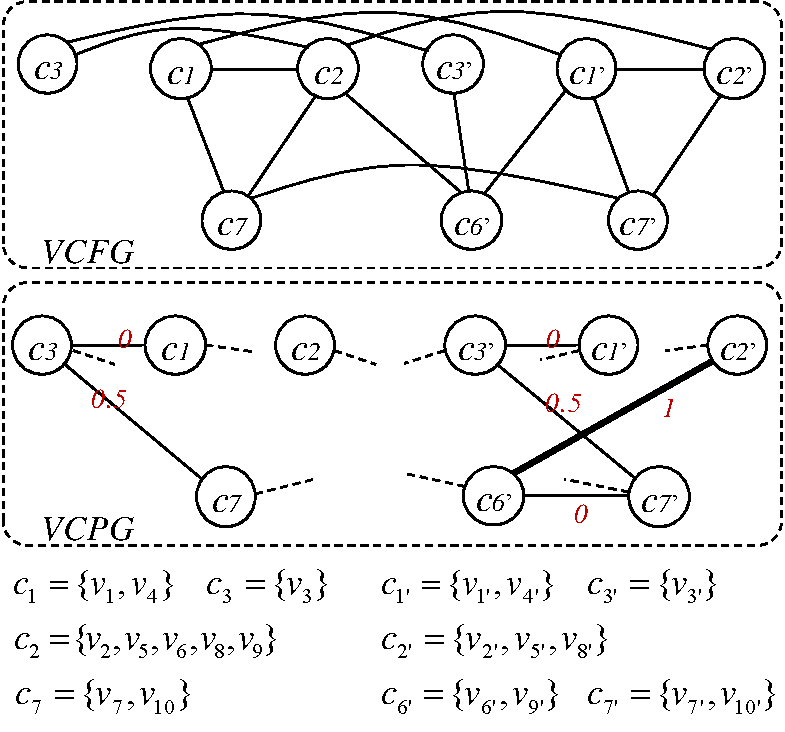
\includegraphics[width=5.8cm]{figure/vcg1.pdf}\label{subfig:assign1}
} &\hspace*{-1.5em}
\subfigure [] {
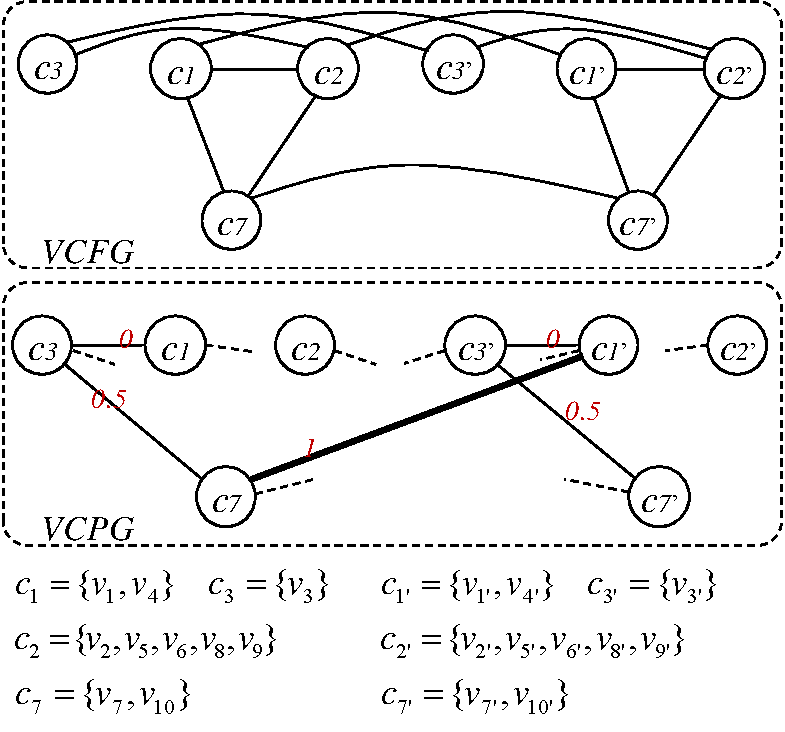
\includegraphics[width=5.8cm]{figure/vcg2.pdf}\label{subfig:assign2}
} &\hspace*{-1.5em}
\subfigure [] {
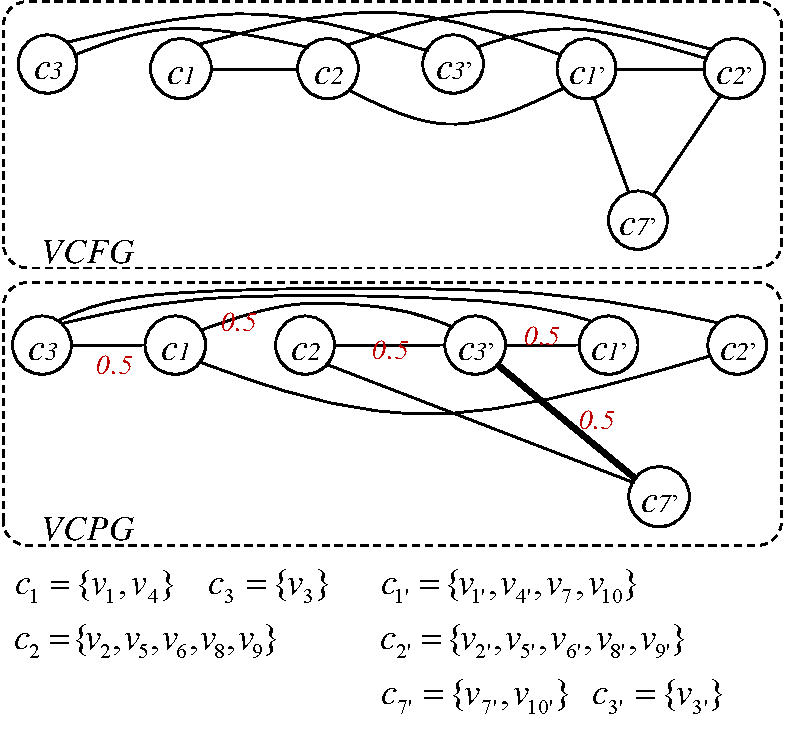
\includegraphics[width=5.8cm]{figure/vcg3.pdf}\label{subfig:assign3}
} \\\hspace*{-1em}
\subfigure [] {
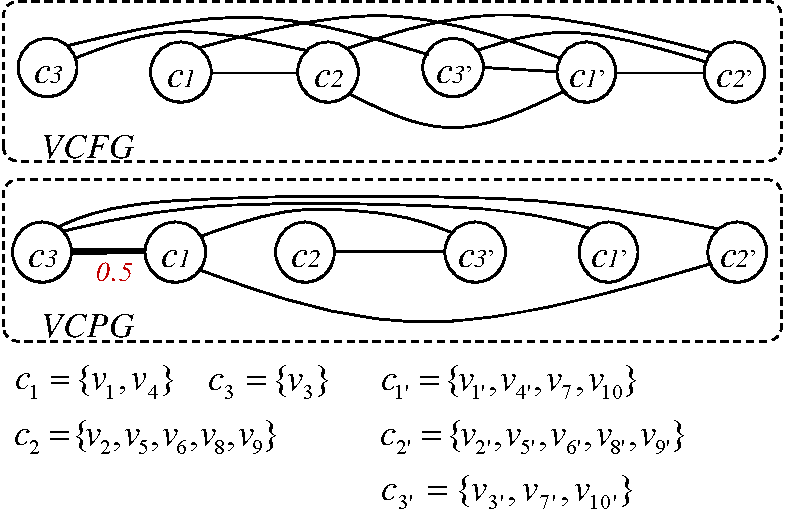
\includegraphics[width=5.8cm]{figure/vcg4.pdf}\label{subfig:assign4}
} &\hspace*{-1.5em}
\subfigure [] {
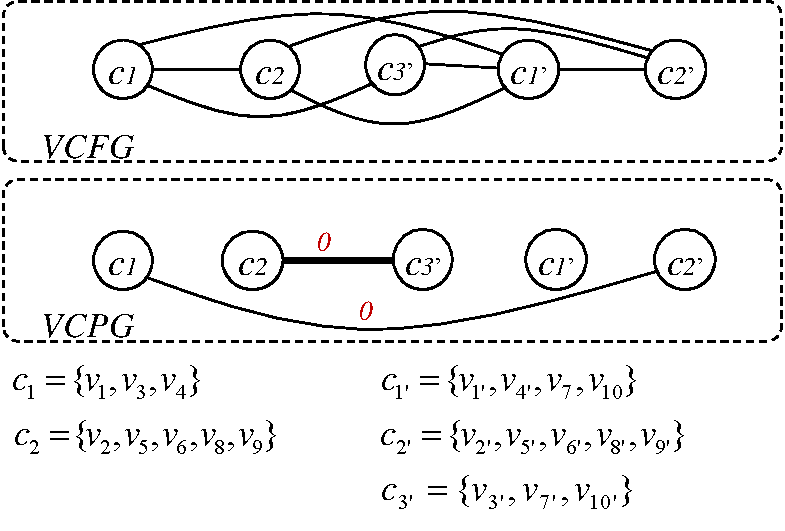
\includegraphics[width=5.8cm]{figure/vcg5.pdf}\label{subfig:assign5}
} &\hspace*{-1.5em}
\subfigure [] {
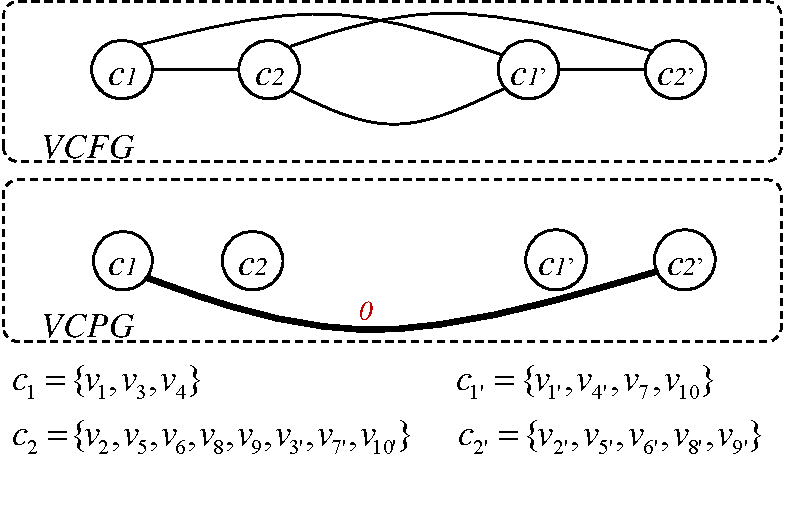
\includegraphics[width=5.8cm]{figure/vcg6.pdf}\label{subfig:assign6}
}
\end{tabular}
\caption{The procedure of vendor assignment. \subref{subfig:assign1} $VCFG$ and $VCPG$ in the 2nd iteration of cluster merging. \subref{subfig:assign2} $VCFG$ and $VCPG$ in the 3th iteration of cluster merging. \subref{subfig:assign3} $VCFG$ and $VCPG$ in the 4th iteration of cluster merging. \subref{subfig:assign4} $VCFG$ and $VCPG$ in the 5th iteration of cluster merging. \subref{subfig:assign5} $VCFG$ and $VCPG$ in the 6th iteration of cluster merging. \subref{subfig:assign6} $VCFG$ and $VCPG$ in the 7th iteration of cluster merging.}
\vspace*{-0.9em}
\label{fig:assign}
\end{figure*}

Larger value of $Merge(c_i, c_j)$ means a higher probability that tasks in $c_i$ and $c_j$ can share the same cores, and therefore, assigning these tasks to the same IP vendor reduces the number of cores. Examples of calculating $Merge(c_2, c_3)$ and $Merge(c_2, c_7)$ are presented in Fig. \ref{subfig:vcg_c_2}. $Merge(c_2, c_3)=1+0.5-1.5=0$, and this means core reduction cannot be obtained from merging $c_2$ and $c_3$. $Merge(c_2, c_7)=1+1-1=1$, indicating that tasks in $c_2$ and $c_7$ can share the same core, and merging $c_2$ and $c_7$ reduces the core usage.

$Merge(c_i, c_j)$ is then set as the weight of edge $(c_i, c_j)$ in $VCPG$, and the edge with maximum weight is chosen and the connected clusters are merged into one.

% Contracting the maximum weight edge in $VCPG$ means the maximization of cores charing, which can in turn minimize the number of cores required.

Algorithm \ref{alg:VA} gives the details of the proposed vendor assignment algorithm. Firstly (\textit{lines: 1-6}), the mobilities of tasks are calculated, and the number of cores required by each cluster is estimated by $DG_{max}(c)$. Secondly (\textit{lines: 7-11}), the $VCFG$ and $VCPG$ are constructed, and the weight of each edge in $VCPG$ is evaluated. Thirdly (\textit{lines: 12-17}), the maximum weight edge in $VCPG$ is chosen, and the connected clusters are merged into one cluster. Both $VCFG$ and $VCPG$ are then updated, and this procedure continues until the number of clusters equals the number of IP vendors available. Finally (\textit{line: 18}), tasks in the same cluster are assigned with the same IP vendor. Considering that $VCPG$ with $O(n)$ nodes has almost $O(n^2)$ edges, the maximum weight independent set of $VCPG$ is not introduced to determine the contracted edges due to the large time complexity, and instead, the edge with maximum weight is iteratively selected and contracted.


\begin{algorithm}[!h]
\caption{Vendor-assignment with core minimization, $vendor\_assign(TC, TC', vc)$.}
\label{alg:VA}
{Input:}
vendor constraint, $vc$; \\
\hspace*{2.8em} performance-constrained clustering results of task\\
\hspace*{2.8em}  graph and duplicated task graph, $TC$, $TC'$.\\
{Output:} vendor assignment, $VA$.
\begin{algorithmic}[1]
\FOR{each node $v$ in $TG$ and $TG'$}
    \STATE calculate the mobility of $v$.
\ENDFOR
\FOR{each cluster $c$}
    \STATE calculate $DG_{max}(c)$.
\ENDFOR
\STATE Construct $VCFG$ from $TC$ and $TC'$;
\STATE Construct $VCPG$ from $VCFG$;
\FOR{each edge $e\in VCPG$}
    \STATE calculate $VCPG.edge\_weight(e)$.
\ENDFOR
\WHILE{$VCPG.node\_num > vc$}
\STATE Choose the edge $e_{max}=(c_i,c_j)$ with the maximum weight in $VCPG$.
\STATE Merge $c_i$ and $c_j$ into one cluster, denoted as $c_{i}$;
\STATE Update $VCFG$ and $VCPG$;
\STATE Calculate $DG_{max}(c_i)$, and update the weights of edges that connect $c_i$ in $VCPG$.
\ENDWHILE
\STATE Each cluster is assigned with one IP vendor.
\end{algorithmic}
\end{algorithm}




An example of vendor assignment procedure is illustrated in Fig. \ref{fig:assign}, where the initial $VCFG$ and $VCPG$ are presented in Fig. \ref{subfig:vcg_c_1}, and the vendor constraint is 3. The maximum weight of all edges in $VCPG$ is 1, and $c_2$ and $c_6$ in Fig. \ref{subfig:vcg_c_1} are merged into one cluster, named $c_2$. All edges that once connect to $c_2$ and $c_6$ in $VCFG$ now connect to $c_2$ in the updated $VCFG$, and the weights of edges that connect to $c_2$ in $VCPG$ will also be updated. Fig. \ref{subfig:assign1} gives the $VCFG$ and $VCPG$ after the 1st iteration of merging clusters. Then, $c_2'$ and $c_6'$ are merged in the 2nd iteration because the weight of their connecting edge is 1, and Fig. \ref{subfig:assign2} presents the updated $VCFG$ and $VCPG$. With the corresponding $VCFG$ and $VCPG$ shown in Fig. \ref{subfig:assign2}-Fig. \ref{subfig:assign6}, the pairs of clusters ($c_1'$, $c_7$), ($c_3'$, $c_7'$), ($c_1$, $c_3$), ($c_2$, $c_3'$) and ($c_1$, $c_2'$) are iteratively merged. Finally, this procedure terminates when the number of clusters equals the vendor constraint, and Fig. \ref{fig:assign_result} gives the final results, whose total estimated number of cores is 5.5. After the cluster merging procedure, tasks in each cluster will be assigned to the same IP vendor.



\begin{figure}[!t]
\centering
\hspace*{-0.8em}
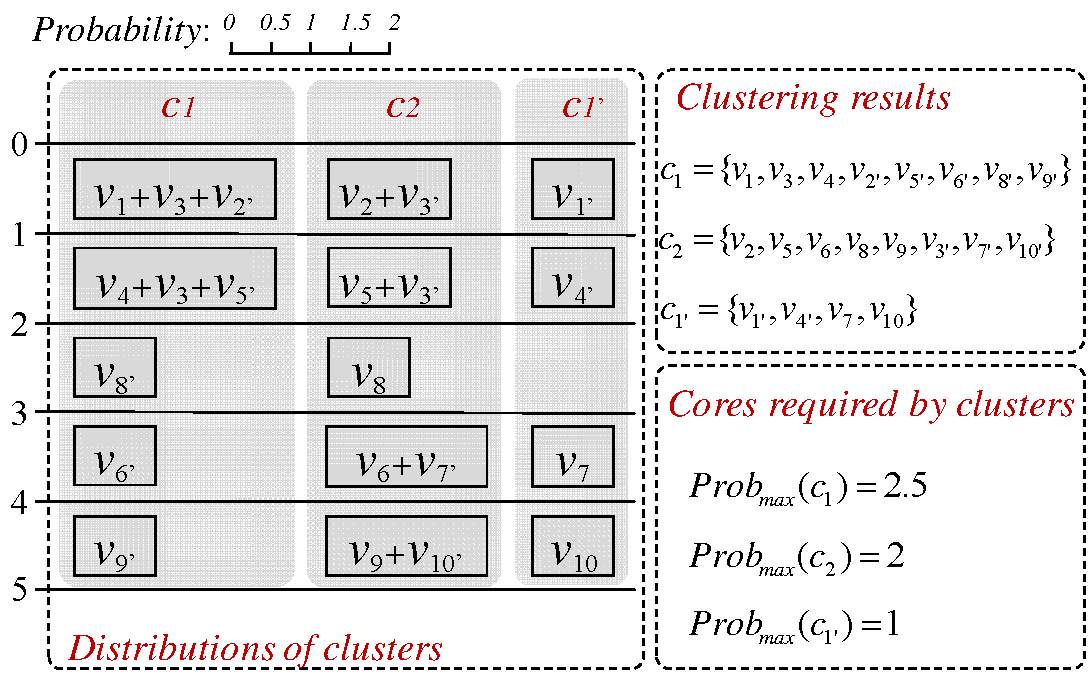
\includegraphics[width=8.8cm]{figure/vcg_result.pdf}
\caption{Cluster merging results with a minimized number of cores required.}
\label{fig:assign_result}
\end{figure}

%The total number of cores required is denoted as $core$, and it is the sum of all estimated cores $core=\sum\limits_{\forall ipv_k}DG_m(ipv_k)$. An example of estimating the total number of cores is given in Fig. \ref{fig:ipv1-1}, with the $VCG$ and the corresponding $vcs$ demonstrated in Fig. \ref{fig:resource_req}. The mobility of each task (presented in Fig. \ref{subfig:mobility1}) is first calculated before constructing the distribution graphs. Then, the distribution graphs of all IP vendors are calculated, and the estimated numbers of cores in each unit of time ($u.t.$) of the 1st, 2nd, 3rd, and 4th IP vendors are shown in Fig.\ref{subfig:dg1-1}, Fig.\ref{subfig:dg1-2}, Fig.\ref{subfig:dg1-3}, and Fig.\ref{subfig:dg1-4}, respectively. The number of cores required by each IP vendor is estimated by the maximum number of $DG$ among all unit of times, and Fig. \ref{subfig:dg1-5} shows the estimated number of cores of each IP vendor, indicating that a total number of 6.42 cores are required during the current vendor assignment.
%\begin{figure}[!t]
%\centering
%\begin{tabular}{cc}
%\hspace*{-1.0em}
%\subfigure [] {
%\includegraphics[width=4.1cm]{figure/mobility1.pdf}\label{subfig:mobility1}
%} &
%\subfigure [] {
%\includegraphics[width=3.6cm]{figure/dg1-1.pdf}\label{subfig:dg1-1}
%} \\ \hspace*{-1.0em}
%\subfigure [] {
%\includegraphics[width=3.6cm]{figure/dg1-2.pdf}\label{subfig:dg1-2}
%} &
%\subfigure [] {
%\includegraphics[width=3.6cm]{figure/dg1-3.pdf}\label{subfig:dg1-3}
%} \\ \hspace*{-1.0em}
%\subfigure [] {
%\includegraphics[width=3.6cm]{figure/dg1-4.pdf}\label{subfig:dg1-4}
%} &
%\subfigure [] {
%\includegraphics[width=3.6cm]{figure/dg1-5.pdf}\label{subfig:dg1-5}
%}
%\end{tabular}
%\caption{Example of core estimation. \subref{subfig:mobility1} Mobilities of tasks. \subref{subfig:dg1-1} The distribution graphs of the 1st vendor. \subref{subfig:dg1-2} The distribution graphs of the 2nd vendor. \subref{subfig:dg1-3} The distribution graphs of the 3rd vendor. \subref{subfig:dg1-4} The distribution graphs of the 4th vendor. \subref{subfig:dg1-5} The estimated number of cores required.}
%\label{fig:ipv1-1}
%\end{figure}





%To assign $c_i$ with the most appropriate IP vendor, we first estimate the number of cores required if $c_i$ is assigned to $ipv_k$, $\forall ipv_k\in cvs(c_i)$, and then assign $c_i$ to the IP vendor with the smallest number of cores required. Fig. \ref{subfig:vcg1} illustrates an example of assigning $c_1$ with proper IP vendor, where $cvs(c_1)=\{ipv_1, ipv_2, ipv_4\}$. The numbers of cores required if $c_1$ is assigned to $ipv_1$, $ipv_2$ and $ipv_4$ are 7.67, 7.33, and 7.33, respectively (see Figs. \ref{subfig:assign2} \ref{subfig:assign3} \ref{subfig:assign4}). Thus, $c_1$ will be assigned to either $ipv_2$ or $ipv_4$, because their vendor assignments are equally evaluated.



%Each time after assigning a cluster with a proper IP vendor, we schedule all of the tasks in this cluster by force-directed scheduling method \cite{article:PP}. Force-directed scheduling method schedules tasks evenly in time periods, resulting in a small number of cores required. Algorithm \ref{alg:PCTS} illustrates the details of our security-Driven performance-constrained task scheduling algorithm.




\subsection{The Procedure of Our Proposed Task Scheduling Method}
%Common input data can be shared between tasks when: 1) these tasks can be assigned to the same core; 2) these tasks have the same parent. Tasks $v_i$ and $v_j$ can be assigned to the same core when the following two situations are both satisfied:
%\begin{enumerate}
%\item $v_i$ and $v_j$ are assigned to the same vendor;
%\item $m_s(v_i)-m_e(v_j)\geq d(v_i)+d(v_j)$, or $m_s(v_j)-m_e(v_i)\geq d(v_i)+d(v_j)$.
%\end{enumerate}

%We assert that $v_i$ and $v_j$ are \textit{compatible} if they can be assigned to the same core. Scheduling a task into a specific $EI$ equals narrowing its mobility, and the mobilities of its ancestors and successors may also be narrowed. This makes two tasks, which were once compatible, no longer able to be assigned to the same core due to the narrowed mobilities.

%Regarding two tasks that consume $k~(u.m.)$ common input data, assigning them to the same core could reduce the amount of data fetched from the off-chip memory by $k~(u.m.)$. The cost of scheduling task $v_i$ into $EI$ on common data sharing is denoted as $cost_{mem}(v_{i}, EI)$, which is calculated as follows.
%\begin{equation}
%cost_{mem}(v_{i}, EI) = \sum\limits_{\forall v_j\in \phi(v_i)} data_{c}(v_i,v_j)
%\label{equ:cost_m}
%\end{equation}

%\noindent where $data_c(v_i,v_j)$ is the total amount of common data that is consumed by both $v_i$ and $v_j$. $\phi(v_i)$ is the set of tasks that were compatible with $v_i$ before scheduling $v_i$ into $EI$ and non-compatible with $v_i$ after scheduling.

%In the example shown in Fig. \ref{fig:TG2}, if $v_3$ is scheduled into [20,25] as shown in Fig. \ref{subfig:TG2-2}, the resulting in $\phi(v_3)$ is $\{v_2\}$, and $cost_{mem}(v_{3}, EI^{v_3}_{20})$ is calculated following Eq. \ref{equ:cost_m}, yielding 10, which means that $10~(u.m.)$ data can no longer be shared between $v_3$ and the tasks in $\phi(v_3)$. If $v_3$ is scheduled into [30,35] as shown in Fig. \ref{subfig:TG2-3}, the resulting $\phi(v_3)$ is $\emptyset$, and thus, $cost_{mem}(v_{3}, EI^{v_3}_{30})=0$. The larger $cost_{mem}$ means that more opportunities for sharing common input data have been discarded, and tasks are tended to be scheduled to the $EI$ with lower cost.
With all security constraints satisfied, the number of IP vendors is always equal the number of nodes in the maximum clique (denoted as \textit{maximum clique size}) of $TG$. However, both the performance-constrained task clustering and vendor assignment may potentially increase the number of vendors needed, and we need to check every contracted edge if the resulting maximum clique size exceed the vendor constraint. Computing the maximum clique size of a graph is NP-complete, and an efficient heuristic approach \cite{article:CL} is introduced in this paper. Each time after determining a contracted edge, the impact on the maximum clique size of the corresponding $VCFG$ is evaluated, and the edge will not be contracted if the vendor constraint is violated. Instead, the algorithm chooses the second best solutions.

After vendor assignment, tasks with the same IP vendor will be scheduled together using force-directed scheduling (FDS) method \cite{article:PP}. FDS tends to schedule tasks evenly in each time period, and only a small number of cores is required. Algorithm \ref{alg:PCTS} gives the whole procedure of the proposed task scheduling algorithm. Tasks in task graph and duplicated task graph are first clustered under the performance constraint $p_c$ (\textit{lines: 1-2}), and they are then assigned to IP vendors with a minimized number of cores required (\textit{lines: 3-4}). Finally, tasks in each IP vendor will be scheduled at the same time by FDS (\textit{lines: 5-9}).


\begin{algorithm}[!h]
\caption{Performance-constrained task scheduling with area optimized, $task\_schedule(TG, pc)$.}
\label{alg:PCTS}
{Input:} task graph, $TG$\\
\hspace*{2.8em}performance constraint, $pc$;\\
{Output:} scheduling results, $TS$.
\begin{algorithmic}[1]
\STATE $TC=task\_cluster(TG,pc)$;
\STATE $TC'=task\_cluster(TG',pc)$, where $TG'$ is the duplicate of $TG$;
\STATE $c_v=max\_clique\_size(TG)$;
\STATE $VA=vendor\_assign(TC, TC', vc)$;
\FOR{each vendor $vendor_i$}
    \STATE $V_{vendor_i}$ is the set of all tasks assigned to $vendor_i$;
    \STATE Calculate the mobilities of tasks in $V_{vendor_i}$;
    \STATE $FDS(V_{vendor_i}, pc)$;% using Force-directed scheduling;
\ENDFOR
\end{algorithmic}
\end{algorithm}

The time complexity of our proposed method is analyzed as follows, and we suppose the input task graph has $n$ nodes and $m$ edges.

In each iteration of performance-constrained task clustering stage, constructing $ECCG$ from $TVG$ needs $O(m^2)$, and finding the MWIS in $ECCG$ also needs $O(m^2)$ \cite{conference:LC}. Only a constant number of iterations are conducted before reaching the performance constraint, and finding all contracted edges to meet the performance constraint totally needs $O(m^2)$. In addition, each time before contracting an edge, updating $VCFG$ and evaluating the impact on the maximum clique size of $VCFG$ need $O(n^2)$, and only a limited number of edges are contracted, making its computational cost to be $O(n^2)$. To sum up, the total time complexity of performance-constrained task clustering is $O(n^2+m^2)$.

In the vendor assignment and task scheduling stage, constructing $VCFG$ and $VCPG$ needs $O(n^2)$. In each iteration of merging clusters, $O(m)$ is required to estimate the maximum clique size, and $O(n)$ is needed to update both $VCFG$ and $VCPG$. Vender assignment needs $O(n)$ iterations of merging clusters, and its time complexity is $O(mn)$. Performing force-directed scheduling method to schedule all tasks needs $O(n^2)$, and the total time complexity of vendor assignment and task scheduling stage is $O(n^2+mn)$.

The sum of $O(n^2+m^2)$ and $O(n^2+mn)$ is $O(n^2+m^2)$ (due to $O(n)\leq O(m)\leq O(n^2)$), and it is the total time complexity of our proposed method.


\section{Experimental Results}

\subsection{Experimental Setups}
All of the experiments were implemented in C on a Linux Workstation with an E5 2.6-GHz CPU and 32-GB RAM. To demonstrate the effectiveness of our proposed algorithms, we tested eight benchmarks from two sources\footnote{https://www.kasahara.cs.waseda.ac.jp/schedule/index.html.}: task graphs that are modeled from actual application programs, including Robot control (robot), Sparse matrix solver (sparse), SPEC fpppp (fpppp); task graphs that are randomly generated (rnc500, rnc1000, rnc2000, rnc3000 and rnc5000). To simplify the experiments, all intra-core communication delays were ignored.

\begin{table}[!h]
\renewcommand{\arraystretch}{1.1}
\caption{Details of the Benchmarks}
\centering
\begin{tabular}{c|c|c|c|c|c|c}
\hline
\hline

task    &\multicolumn{1}{c|}{\multirow{2}{*}{nodes}}     &\multicolumn{1}{c|}{\multirow{2}{*}{edges}}     &\multicolumn{1}{c|}{\multirow{2}{*}{Para. }}  &ACC  &\multicolumn{1}{c|}{\multirow{2}{*}{$scy$}}   &maximum  \\
graph   &                                            &           &        & ($u.t.$)     &      & clique size       \\
\hline
\hline

robot   &88   &131     &4.4 &28.2  &350 &3 \\

sparse  &96   &67    &16.0  &20.2 &230  &3 \\

fpppp   &334   &1145    &6.7  &21.3 &2624   &3  \\

rnc500  &500   &1910    &27.7  &10.6  &4320  &3  \\

rnc1000  &1000   &3005   &60.2  &7.8 &7010 &3 \\

rnc2000   &2000   &3930   &151.9  &10.6 &9860  &3 \\

rnc3000   &3000   &39034    &34.2 &13.0 &81068  &4  \\

rnc5000   &5000   &55432   &90.8  &11.0 &115864 &4 \\

\hline
\hline
\end{tabular}
\label{table:detail}
\end{table}

%To test the performance of our proposed methods, a set of benchmarks is tested, and

Table I shows the details of these benchmarks. The columns nodes and edges give the numbers of tasks and communications in each task graph, respectively. Column Para. shows the parallelism of each task graph, which is the ratio of the total processing time of all tasks to the ASAP schedule length (without communication delay). Column ACC gives the averaged computational cost of each task, and column $scy$ gives the total number of security constraints. Considering that the maximum clique sizes of most task graphs modeled from actual application programs are no larger than 4\cite{article:CL}, the maximum clique sizes of all randomly generated $TG$ we tested in the experiments are 3 or 4.
%\begin{enumerate}
%\item Comparing the benchmarks with the same number of nodes, the benchmark with larger maximum clique size always indicates a larger number of edges. Therefore, too many edges have to be contracted to boost the performance, which is not practical in actual.
%\item The maximum clique sizes of most task graphs are no larger than 4\cite{article:CL}.
%\end{enumerate}


%To demonstrate the effectiveness of our proposed methods, the task scheduling results of our methods are compared with a Baseline method \cite{article:CL} which schedules task strictly following the security constraints.

Our proposed \textit{MWIS-based} method is then compared with another two methods. The \textit{list-based} method proposed in \cite{article:CL} optimizes the schedule length by placing critical tasks on a single core, and conducts IP vendor assignment using traditional coloring method. The \textit{min-cut-based} method proposed in \cite{article:NW} boosts the performance by iteratively contracting the edges selected by max-flow min-cut algorithm, and assigns tasks with IP vendors while considering the core speed variation.



\subsection{Performance Optimization Results Without Trojan Attack Probability Variation}



%Since both \textit{list-based} and \textit{min-cut-based} methods ignore the Trojan attack probability variations, and we first assume that the Trojan attack probabilities are the same among all edges. Therefore, Optimizing the attack risk equals to minimize the $scy_v$.

The IP vendor constraint is set to be the maximum clique size of benchmark. The \textit{communication-to-computation ratio} ($CCR$) is the ratio of the inter-core communication delay to the computational cost of the task, and $CCR$ is set to be 1.0 in this set of experiments. Since both \textit{list-based} and \textit{min-cut-based} methods ignore the Trojan attack probability variation, and Trojan attack probabilities of all communications are assumed to be the same in this set of experiments. Therefore, maximizing the system security is equivalent to minimizing the number of security constraint violations (denoted as $scy_v$).

\begin{table}[!h]
\renewcommand{\arraystretch}{1.1}
\caption{Performance Optimization Results Without Trojan Attack Probability Variation.}
\centering
\begin{tabular}{c|c|c|c|c|c|c|c|c}
\hline
\hline
task                             &SL           &$c_p$        & \multicolumn{2}{c|}{\textit{list-based}}        &\multicolumn{2}{c|}{\textit{min-cut-based}}   &\multicolumn{2}{c}{\textit{MWIS-based}}        \\  \cline{4-5} \cline{6-7} \cline{8-9}
graph                                                   &\hspace*{-1em}($u.t.$)\hspace*{-1em}         &($u.t.$)       &\hspace*{-1em}$scy_v$\hspace*{-1em}     & \hspace*{-0.6em}$ratio(\%)$\hspace*{-0.6em}  &$scy_v$     &\hspace*{-0.6em}$ratio(\%)$\hspace*{-0.6em}   &\hspace*{-1em}$scy_v$\hspace*{-1em}     &\hspace*{-0.6em}$ratio(\%)$\hspace*{-0.6em}   \\

\hline
\hline

\multicolumn{1}{c|}{\multirow{2}{*}{robot}}               &\multicolumn{1}{c|}{\multirow{2}{*}{\hspace*{-1em}1114\hspace*{-1em}}}      &997  &10     &2.85   &6   &1.71   &6   &1.71    \\
   &      &892   &24  &6.86  &16   &4.57    &16  &4.57 \\

\hline
\multicolumn{1}{c|}{\multirow{2}{*}{sparse}}              &\multicolumn{1}{c|}{\multirow{2}{*}{236}}        &208  &4  &1.74   &2   &0.87    &2   &0.87   \\
   &     &192   &6  &2.61  &4   &1.74  &4    &1.74  \\

\hline
\multicolumn{1}{c|}{\multirow{2}{*}{fpppp}}            &\multicolumn{1}{c|}{\multirow{2}{*}{\hspace*{-1em}2119\hspace*{-1em}}}  &\hspace*{-0.5em}1871\hspace*{-0.5em}  &6 &0.24  &2   &0.08  &2   &0.08  \\
   &       &\hspace*{-0.5em}1623\hspace*{-0.5em}   &8 &0.30   &4   &0.16  &4  &0.15 \\

\hline
\multicolumn{1}{c|}{\multirow{2}{*}{\hspace*{-0.5em}rnc500\hspace*{-0.5em}}}            &\multicolumn{1}{c|}{\multirow{2}{*}{373}}    &340   &6  &0.14  &4  &0.09   &4  &0.09   \\
  &     &300  &26  &0.60  &18   &0.42  &18  &0.42 \\

\hline
\multicolumn{1}{c|}{\multirow{2}{*}{\hspace*{-1em}rnc1000\hspace*{-1em}}}              &\multicolumn{1}{c|}{\multirow{2}{*}{254}}   &226    &16 &0.23   &12   &0.17 &12   &0.17  \\
   &     &203   &86  &1.23  &64  &0.91  &62  &0.88 \\

\hline
\multicolumn{1}{c|}{\multirow{2}{*}{\hspace*{-1em}rnc2000\hspace*{-1em}}}            &\multicolumn{1}{c|}{\multirow{2}{*}{268}}    &243    &14  &0.14  &8   &0.08  &8 &0.08   \\
  &    &219   &52  &0.53  &38    &0.38  &38 &0.38  \\

\hline
\multicolumn{1}{c|}{\multirow{2}{*}{\hspace*{-1em}rnc3000\hspace*{-1em}}}           &\multicolumn{1}{c|}{\multirow{2}{*}{\hspace*{-1em}1779\hspace*{-1em}}}  &1601  &186  &0.23  &132   &0.16   &\hspace*{-1em}132\hspace*{-1em}   &0.16  \\
   &     &1423   &\hspace*{-1em}1340\hspace*{-1em}  &1.65   &982   &1.21   &984  &1.21 \\

\hline
\multicolumn{1}{c|}{\multirow{2}{*}{\hspace*{-1em}rnc5000\hspace*{-1em}}}           &\multicolumn{1}{c|}{\multirow{2}{*}{\hspace*{-1em}1146\hspace*{-1em}}}    &1031  &826  &0.71  &534  &0.46   &\hspace*{-1em}528\hspace*{-1em}  &0.46     \\
   &     &917   &\hspace*{-1em}2396\hspace*{-1em}   &2.07   &\hspace*{-1em}1784\hspace*{-1em}   &1.54   &\hspace*{-1em}1778\hspace*{-1em}  &1.54  \\

\hline
\multicolumn{1}{c|}{\multirow{2}{*}{\hspace*{-1em}avg.\hspace*{-1em}}}           &\multicolumn{1}{c|}{\multirow{2}{*}{}}    &\hspace*{-1em}0.9SL\hspace*{-1em}  &   &0.79   &  &0.45   &   &0.45    \\
   &     &\hspace*{-1em}0.8SL\hspace*{-1em}   &    &1.98    &   &1.36   &   &1.36  \\
\hline
\hline
\end{tabular}
\label{table:VPCTC}
\end{table}



Table II gives the comparison results without Trojan attack probability variation, and the ratio of $scy_v$ to $scy$ is used to evaluate the system risk, which is given in column $ratio$. The performance constraint $pc$ is set as $pc=\mathrm{\delta*SL}$, where $\mathrm{SL}$ is the ASAP schedule length with all security constraints satisfied. Two performance constraints are tested for each benchmark, with $\delta \in \{0.9, ~0.8\}$. The results show that \textit{list-based} method violates the $0.79\%$, and $1.98\%$ security constraints, when $\delta$ is set to be 0.9 and 0.8, respectively. The $scy_v$ optimization results of \textit{min-cut-based} and \textit{MWIS-based} are almost the same in all benchmarks, and the ratios of $scy_v$ to $scy$ are $0.45\%$ and $1.36\%$ when $\delta$ is set to be 0.9 and 0.8, respectively.

The above results indicate that the number of violated security constraints is very limited if the schedule length is optimized to $0.9\mathrm{SL}$, and this number significantly increases if the schedule length is further reduced from $0.9\mathrm{SL}$ to $0.8\mathrm{SL}$. Therefore, the schedule length should not be over optimized, otherwise the system will face large Trojan attack risks.

\subsection{Performance Optimization Results With Trojan Attack Probability Variation}

Then, the Trojan attack probability variation between communications are counted. We assume that the task outputs may contain more confidential information and the Trojan attack damage to the system become more serious when the application proceeds. Therefore, the probability that Trojan attack via edge $e_{ij}$ in $TG$ or $TG'$ is set to be $risk(e_{ij})=dis(e_{ij})/|E|$ in this set of experiments, where $dis(e_{ij})$ is the distance from $s$ to $v_i$ and $|E|$ is the number of edges. The system risk is given in column $risk_s$, and the performance constraint $p_c$ is set to be $0.9\mathrm{SL}$.


\begin{table}[!h]
\renewcommand{\arraystretch}{1.1}
\caption{Performance Optimization Results With Trojan Attack Probability Variation.}
\centering
\begin{tabular}{c|c|c|c|c|c|c|c|c|c}
\hline
\hline
\multirow{2}{*}{task}                  &\multirow{2}{*}{$pc$}        & \multicolumn{2}{c|}{\textit{list-based}}        &\multicolumn{3}{c|}{\textit{min-cut-based}}   &\multicolumn{3}{c}{\textit{MWIS-based}}        \\  \cline{3-4} \cline{5-7} \cline{8-10}
\multirow{2}{*}{graph}                 &\multirow{2}{*}{\hspace*{-1em}($u.t.$)\hspace*{-1em}}       &\multirow{2}{*}{\hspace*{-0.6em}$scy_v$\hspace*{-0.6em}}     & \hspace*{-0.6em}$risk_s$\hspace*{-0.6em}  &\multirow{2}{*}{\hspace*{-0.6em}$scy_v$\hspace*{-0.6em}}     &\hspace*{-0.6em}$risk_s$\hspace*{-0.6em}  &\hspace*{-0.4em}$redu_{r}$\hspace*{-0.4em}  &\multirow{2}{*}{\hspace*{-0.6em}$scy_v$\hspace*{-0.6em}}      &\hspace*{-0.6em}$risk_s$\hspace*{-0.6em}  &\hspace*{-0.4em}$redu_{r}$\hspace*{-0.4em}  \\
    &       &     & \hspace*{-0.8em}$(10^{-3})$\hspace*{-0.8em}  &     &\hspace*{-0.8em}$(10^{-3})$\hspace*{-0.8em} &(\%)   &     &\hspace*{-0.6em}$(10^{-3})$\hspace*{-0.6em} &(\%)   \\

\hline
\hline

robot                   &997  &10     &142.60   &6   &60.69 &\hspace*{-0.8em}57.44\hspace*{-0.8em}  &6   &38.02  &\hspace*{-0.8em}73.34\hspace*{-0.8em}   \\
%   &      &892   &24  &  &16   &56.46    &18  &34.44 \\


\hspace*{-1em}sparse\hspace*{-1em}                    &208  &4  &118.66   &2   &89.25  &\hspace*{-0.8em}24.78\hspace*{-0.8em}  &2   &74.48 &\hspace*{-0.8em}37.23\hspace*{-0.8em}  \\
%   &     &192   &6  &  &4   &21.82  &4    &21.82  \\


\hspace*{-1em}fpppp\hspace*{-1em}             &\hspace*{-1em}1871\hspace*{-1em}  &6 &24.18  &2   &19.11  &\hspace*{-0.8em}20.98\hspace*{-0.8em} &2   &15.65 &\hspace*{-0.8em}35.28\hspace*{-0.8em} \\
%   &       &\hspace*{-0.5em}1623\hspace*{-0.5em}   &8 &   &4   &41.24  &4  &37.46 \\


\hspace*{-1em}rnc500\hspace*{-1em}        &340   &6  &19.59  &4  &12.45 &\hspace*{-0.8em}36.43\hspace*{-0.8em}  &4  &8.32 &\hspace*{-0.8em}57.50\hspace*{-0.8em} \\
%  &     &300  &26  &  &18   &160.50  &22  &113.43 \\


\hspace*{-1em}rnc1000\hspace*{-1em}              &226    &16 &30.55  &12   &24.44  &\hspace*{-0.8em}20.02\hspace*{-0.8em}  &14  &18.79 &\hspace*{-0.8em}38.49\hspace*{-0.8em}  \\
%   &     &203   &86  &  &64   &  &68  & \\


\hspace*{-1em}rnc2000\hspace*{-1em}            &243    &14  &22.85  &8      &12.90  &\hspace*{-0.8em}43.54\hspace*{-0.8em}  &10 &8.99  &\hspace*{-0.8em}60.64\hspace*{-0.8em} \\
%  &    &219   &52  &  &38     &  &42 &  \\



\hspace*{-1em}rnc3000\hspace*{-1em}           &\hspace*{-1em}1601\hspace*{-1em}  &\hspace*{-0.5em}186\hspace*{-0.5em}  &\hspace*{-0.5em}11.74\hspace*{-0.5em}  &\hspace*{-0.5em}132\hspace*{-0.5em}   &\hspace*{-0.8em}9.45\hspace*{-0.8em}  &\hspace*{-0.8em}19.54\hspace*{-0.8em}  &\hspace*{-0.5em}144\hspace*{-0.5em}   &\hspace*{-0.8em}8.36\hspace*{-0.8em}  &\hspace*{-0.8em} 28.90 \hspace*{-0.8em} \\
%   &     &243   &98  &   &86   &   &88  & \\



\hspace*{-1em}rnc5000\hspace*{-1em}             &\hspace*{-1em}1031\hspace*{-1em}  &\hspace*{-0.5em}826\hspace*{-0.5em}  &\hspace*{-0.5em}47.77\hspace*{-0.5em}  &\hspace*{-0.5em}534\hspace*{-0.5em}  &\hspace*{-1em}35.19\hspace*{-1em}   & \hspace*{-0.8em}26.32\hspace*{-0.8em} &\hspace*{-0.5em}568\hspace*{-0.5em}  &\hspace*{-1em}31.91\hspace*{-1em}  &\hspace*{-0.8em}33.20\hspace*{-0.8em}  \\


\hline

avg.               &  &   &   &  &  &\hspace*{-0.8em}31.13\hspace*{-0.8em}  &   &  &\hspace*{-0.8em}45.57\hspace*{-0.8em}  \\
%   &     &\hspace*{-1em}0.8SL\hspace*{-1em}   &    &    &   &   &   &  \\
\hline
\hline
\end{tabular}
\label{table:VPCTC}
\end{table}

Table III illustrates the comparison results of these three methods. Because Trojan attack probability variation are not considered in both \textit{list-based} and \textit{min-cut-based}, their task clustering results shown in Table II and Table III are the same. Our proposed \textit{MWIS-based} method minimizes the system risk, and although the $scy_v$ in Table III is slightly increased than that in Table II, the averaged $risk_s$ is significantly reduced. Columns $redu_r$ gives the system risk reduction if compared to \textit{list-based} method, and the averaged system risks of \textit{min-cut-based} and \textit{MWIS-based} methods are 31.13\% and 45.57\% less than \textit{list-based} method, respectively, indicating that \textit{MWIS-based} method maintains the highest security level among all three methods.




\begin{table*}[!t]
\renewcommand{\arraystretch}{1.1}
\caption{Comparisons of Performance-Constrained Task Scheduling Results Without Trojan Attack Probability Variation.}
\centering
\begin{tabular}{c|c|c|c|c|c|c|c|c|c|c|c|c|c|c|c}
\hline
\hline
task                 &\multicolumn{1}{c|}{\multirow{2}{*}{$scy$}}                     &\multicolumn{1}{c|}{\multirow{2}{*}{$CCR$}}     &SL    & $pc$              &\multicolumn{3}{c|}{\textit{list-based}}        &\multicolumn{4}{c|}{\textit{min-cut-based}}    &\multicolumn{4}{|c}{\textit{MWIS-based}}    \\ \cline{6-8} \cline{9-12} \cline{13-16}
graph           &    &   &($u.t.$)   &($u.t.$)    &\multicolumn{1}{c|}{\multirow{1}{*}{$scy_v$}} &\hspace*{-0.4em}$ratio(\%)$\hspace*{-0.4em}    &$core$   &$scy_v$       &\hspace*{-0.4em}$ratio(\%)$\hspace*{-0.4em}  &$core$ &\hspace*{-0.4em}$redu_{c}(\%)$\hspace*{-0.4em}  &$scy_v$       &\hspace*{-0.4em}$ratio(\%)$\hspace*{-0.4em}   &$core$   &\hspace*{-0.4em}$redu_{c}(\%)$\hspace*{-0.4em} \\

\hline
\hline

\multicolumn{1}{c|}{\multirow{2}{*}{robot}}      &\multicolumn{1}{c|}{\multirow{2}{*}{350}} &0.5 &839 &671 &28   &8.00   &14  &18 &5.14  &12   &14.29  &18  &5.14  &11        &21.43 \\
                                              &                                &1.0  &1114  &892  &24 &6.86  &14  &16 &4.57    &12  &14.29  &16 &4.57  &10       &28.57     \\
\hline

\multicolumn{1}{c|}{\multirow{2}{*}{sparse}}    &\multicolumn{1}{c|}{\multirow{2}{*}{230}}  &0.5 &179 &143 &6  &2.61  &21  &4 &1.74  &18  &14.29  &4     &1.74 &16        &23.81 \\
&     &1.0 &236  &189  &6   &2.61   &19  &4 &1.74  &18   &5.26 &4   &1.74   &15      &21.05 \\

\hline

\multicolumn{1}{c|}{\multirow{2}{*}{fpppp}}     &\multicolumn{1}{c|}{\multirow{2}{*}{2624}}   &0.5 &1590  &1272  &10  &0.38 &13  &4 &0.15  &12 &7.70  &4   &0.15   &10        &23.08  \\
&   &1.0 &2119  &1695  &8   &0.30   &12  &4 &0.15 &11  &8.33  &4   &0.15  &10       &16.67  \\

\hline

\multicolumn{1}{c|}{\multirow{2}{*}{\hspace*{-0.5em}rnc500\hspace*{-0.5em}}}    &\multicolumn{1}{c|}{\multirow{2}{*}{4320}}   &0.5 &280  &224  &32   &0.74   &68 &20 &0.46  &65   &4.41 &20  &0.46   &58       &14.71  \\
&    &1.0 &373  &300  &26   &0.60   &67  &20 &0.46  &63  &6.00  &18 &0.42  &56     &16.42       \\

\hline

\multicolumn{1}{c|}{\multirow{2}{*}{\hspace*{-1em}rnc1000\hspace*{-1em}}}     &\multicolumn{1}{c|}{\multirow{2}{*}{7010}}  &0.5 &190  &152  &96   &1.37  &95 &68 &0.97 &88 &7.37  &68  &0.97   &78        &17.89   \\
&   &1.0 &254  &203  &86   &1.23   &87  &64 &0.91 &81   &6.90  &62   &0.88  &74       &14.94  \\

\hline

\multicolumn{1}{c|}{\multirow{2}{*}{\hspace*{-1em}rnc2000\hspace*{-1em}}}    &\multicolumn{1}{c|}{\multirow{2}{*}{9860}} &0.5  &199  &159  &54   &0.55   &217  &42 &0.43 &184 &15.21   &42   &0.43   &167      &23.04 \\
  &   &1.0 &268  &214  &52   &0.53   &206   & 38 &0.39 &180  &12.62   &38   &0.39  &164        &20.39 \\

\hline

\multicolumn{1}{c|}{\multirow{2}{*}{\hspace*{-1em}rnc3000\hspace*{-1em}}}     &\multicolumn{1}{c|}{\multirow{2}{*}{81068}}   &0.5  &1336  &1069  &1468    &1.81    &73   &1126  &1.39  &67 &8.22  &1126    &1.39   &62      &15.07  \\
   &    &1.0 &1779  &1423  &1340   &1.65   &68    &982  &1.21 &62   &8.82   &984   &1.21   &56       &17.65 \\

\hline

\multicolumn{1}{c|}{\multirow{2}{*}{\hspace*{-1em}rnc5000\hspace*{-1em}}}       &\multicolumn{1}{c|}{\multirow{2}{*}{115864}} &0.5   &850  &680  &2560    &2.21   &142  &1964  &1.70  &132  &7.04   &1956   &1.69   &122  &14.08  \\
                                    &             &1.0                                      &1146  &917  &2396   &2.07   &137 &1784 &1.54 &125   &8.76   &1778   &1.54   &115      &16.06   \\

\hline
\multicolumn{1}{c|}{\multirow{2}{*}{avg.}}     & &0.5 &      &  &  &2.21     &  & &1.50 &   &9.82  &   &1.49  & &19.14 \\
                                               &  &1.0 &     &  &  &1.98     &  & &1.38 &   &8.87  &    &1.37  &  &18.97 \\

\hline
\hline
\end{tabular}
\label{table:PCTS}
\end{table*}





\subsection{Comparisons of Task Scheduling Results}



\textit{List-based} method ignores the core optimization, and \textit{min-cut-based} method only saves the core usages when scheduling tasks. In our proposed \textit{MWIS-based} method, reducing the number of cores is considered in both vendor assignment and task scheduling, which enlarges the optimization space of core usages.

To show the effectiveness of our method in saving the number of cores required, the performance constraint is first set to be $\mathrm{SL}$, so that the performance optimization stage can be skipped. Fig. \ref{fig:core_optimization} shows comparison results of core usages, and our proposed \textit{MWIS-based} needs the least number of cores among all benchmarks. \textit{Min-cut-based} and \textit{MWIS-based} methods reduce 7.55\% and 17.92\% core usages if compared to \textit{list-based} method, respectively.%, and our proposed \textit{MWIS-based} needs the least number of cores.
\begin{figure}[!h]
\centering
\hspace*{-1.2em}
\includegraphics[width=9.6cm]{figure/core_optimization.eps}
\caption{Core usages of vendor assignment and task scheduling results.}
\label{fig:core_optimization}
\end{figure}

Then, the performance-constrained task scheduling results are tested, and the results are presented in Table IV. Two $CCRs$ (0.5 and 1.0) are tested, and the Trojan attack probability variation among edges are ignored. The performance constraint is set to be $pc=\mathrm{0.8SL}$, and $ratio$ is the ratio of $scy_v$ to $scy$. Column $core$ gives the numbers of cores required by the scheduling results, and column $redu_{c}$ shows the percentage of reduced core usages if compared to \textit{list-based} method.

The comparison results show that our proposed \textit{MWIS-based} method maintains most of the security constraints and requires the least number of cores. When $CCR=0.5$, our \textit{MWIS-based} reduces $scy_v$ by $0.72\%$ if compared against the \textit{list-based} method, and the number of cores required is $19.14\%$ less. When $CCR=1.0$, the $scy_v$ and $core$ of our \textit{MWIS-based} are 0.61\% and 18.97\% less than \textit{list-based} method, respectively.


% The scheduling results of the clustered-based task scheduling method \cite{article:CL} and our proposed task scheduling method are compared in Table \ref{table:PCTS}, and columns \textit{Cluster} and \textit{TS} demonstrate their scheduling results, respectively. Two $CCRs$ (0.5 and 1.0) are tested, and the task criticality variations are ignored. The performance constraint is set to be $P_c=\mathrm{0.8SL}$, $ratio$ is the ratio of $scy_v$ to $scy$, and $core$ is the total number of cores required by the scheduling result.



%The comparison results show that, when $CCR=0.5$, our $TS$ reduces $scy_v$ by $0.35\%$ if compared against the cluster-based method; In addition, the number of cores required by our $TS$ is $19.18\%$ less than the cluster-based method. When $CCR=1.0$, our $TS$ saves $scy_v$ and $core$ by 0.30\% and 18.59\%, respectively. The runtime of our $TS$ is about 10 times larger than the cluster-based method, but the time complexities of these two methods are both $O(n^3)$, where $n$ is the number of tasks in $TG$.



%and the performance constraint $P_c$ is set as $P_c=\mathrm{\delta*SL}$, where $\mathrm{SL}$ is the ASAP schedule length with all security constraints satisfied. Two performance constraints are tested for each benchmark, with $\delta \in \{0.9, ~0.8\}$. The results show that $TC_1$ violates the minimum number of security constraints, and its $scy_v$ is reduced by 0.24\% if compared against the cluster-based method. $TC_2$ considers the task criticality variations while clustering, and its average $scy_v$ is $0.20\%$ less than that of cluster-based method.


\subsection{Runtime Comparisons}


Finally, the runtimes of \textit{list-based}, \textit{min-cut-based} and \textit{MWIS-based} methods are compared. The time complexity of our proposed \textit{MWIS-based} method is $O(n^2+m^2)$, and in the benchmarks shown in Table I, $m$ can be regarded as $m=cn$, where $c$ is a constant. Therefore, the time complexities of all three methods can be regarded as $O(n^2)$.

\begin{table}[!h]
\renewcommand{\arraystretch}{1.1}
\caption{Comparisons of runtime.}
\centering
\begin{tabular}{c|c|c|c|c|c|c|c}
\hline
\hline
task                             &SL           &$pc$        & \hspace*{-0.5em}\textit{list-based}\hspace*{-0.5em}        &\multicolumn{2}{c|}{\textit{min-cut-based}}   &\multicolumn{2}{c}{\textit{MWIS-based}}        \\  \cline{5-6} \cline{7-8}
graph                                                   &\hspace*{-1em}($u.t.$)\hspace*{-1em}         &($u.t.$)       &$rt(s)$       &$rt(s)$    &$cmp$   &$rt(s)$     &$cmp$    \\
\hline
\hline

robot              &1114      &892  &3.2     &16.3         &5.09 &18.2  &5.69     \\


sparse              &236       &192  &4.8  &37.7       &7.85   &31.7  &6.60   \\

fpppp           &2119  &1623  &7.2 &48.3   &6.71 &49.4    &6.86  \\

rnc500            &373    &300   &17.2  &107.6   &6.26  &97.1   &5.65  \\

rnc1000            &254  &203    &36.3 &247.3  &6.81   &176.3    &4.86   \\

rnc2000          &268    &219    &53.8  &697.3      &12.96   &548.6  &10.20   \\

rnc3000           &1779  &1423  &168.7  &\hspace*{-0.5em}3278.5\hspace*{-0.5em}  &19.43  &\hspace*{-0.5em}2923.3\hspace*{-0.5em}    &17.33  \\

rnc5000          &1146   &917  &368.9  &\hspace*{-0.5em}8786.3\hspace*{-0.5em}  &23.82  &\hspace*{-0.5em}6305.7\hspace*{-0.5em}   &17.09    \\

\hline

avg.          &    &  &   &   &11.12  &   &9.29       \\
\hline
\hline
\end{tabular}
\label{table:VPCTC}
\end{table}



Table V presents the runtime comparison results, where $CCR$ is set to be 1, and $pc=0.8\mathrm{SL}$. Column $rt$ shows the runtimes, and column $cmp$ illustrates the times of runtime if compared to \textit{list-based} method. The averaged comparison results show that the runtimes of \textit{min-cut-based} and \textit{MWIS-based} methods are $11.12$ and $9.29$ times larger than \textit{list-based} method, respectively, and the runtimes of all three methods increase exponentially with the size of input task graph.

In addition, we also tested 20 random generated tasks graphs to show the effects to the runtimes due to different number of edges. All the tested task graphs have 1000 nodes, but the number of their edges ranges from 5000 to 100000. The number of nodes $n$ can be regarded as a constant in this set of experiments, and the time complexities of \textit{min-cut-based} and \textit{MWIS-based} methods become $O(m^2)$, while the time complexity of \textit{list-based} method is only $O(m)$.
\begin{figure}[!h]
\centering
\hspace*{-1.2em}
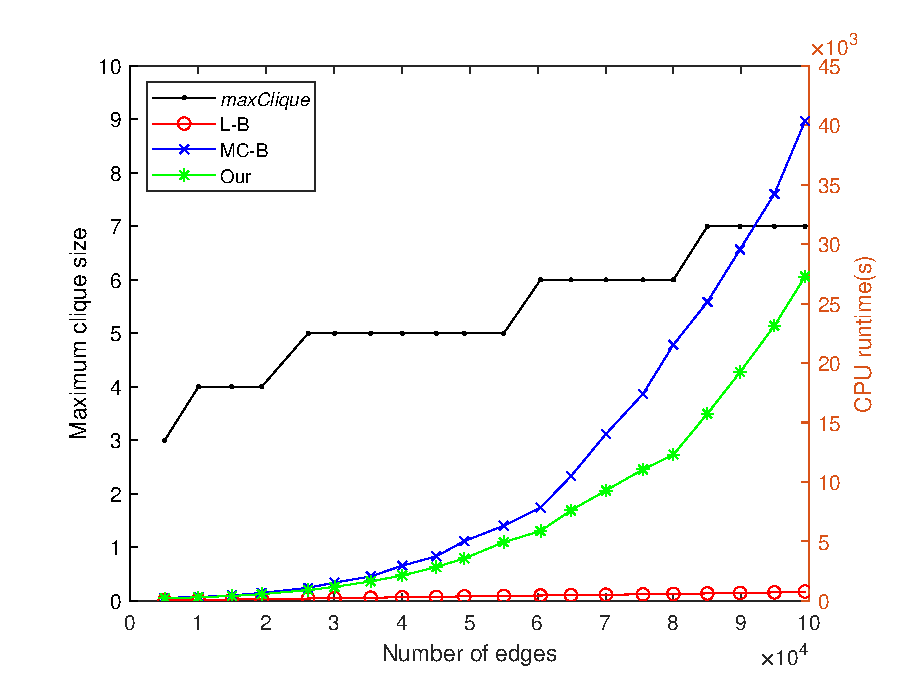
\includegraphics[width=8.1cm]{figure/cpu_runtime.eps}
\caption{CPU runtime comparisons of the three methods when performing 20 random generated task graphs with different number of edges.}
\label{fig:cpu_runtime}
\end{figure}

The runtimes of performing 20 random generated task graphs using \textit{list-based}, \textit{min-cut-based} and \textit{MWIS-based} methods are presented in Fig. \ref{fig:cpu_runtime}. The performance constraint is set to be $pc=0.9\mathrm{SL}$, and the vendor constraint is set to be the maximum clique size of each task graph. The results show that the runtimes of \textit{min-cut-based} and \textit{MWIS-based} methods increase exponentially with the increment of edges, and their runtimes are larger than \textit{list-based} method when the benchmark contains more edges. But the runtimes of our proposed \textit{MWIS-based} method are acceptable when conducting the task graphs whose maximum clique sizes are no larger than 4, and this indicates the efficiency of our proposed method in dealing with the task graphs modeled from actual application programs.

%Column ``$P_c$'' gives the performance constraint that the schedule lengths of both $TG$ and $TG'$ must not exceed. In this set of experiments, we ignore the core-speed variation between vendors, and assume that 1 ($u.t.$) requires $1ms$ to execute. Each task is bound to the appropriate core following the max-cost flow-based binding algorithm \cite{conference:JC} after task scheduling. Column ``$\mathrm{FD_A}$'' gives the amount of data fetched from off-chip memory generated by the Baseline method \cite{article:CL}, and the amount of data fetched from the off-chip memory generated by our proposed method is given in column ``$\mathrm{FD_B}$''. Column ``ratio3'' gives the ratio of $\mathrm{FD_B}$ to $\mathrm{FD_A}$, and column ``runtime'' gives the runtime of vendor assignment and task scheduling (the runtime of task clustering is excluded). Column ``number of cores'' gives the number of cores required to execute all the tasks in both $TG$ and $TG'$. For the actual applications, the number of cores integrated in a MPSoC is limited; and for those randomly generated task graph whose scales are quite large, the resulting number of cores required is also large, and this can be realized by Network on Chip.

%Both the number of cores required and the amount of data fetched from off-chip memory are simultaneously optimized in the task scheduling stage, and the amount of fetched data in $\mathrm{TS_1}$ is $15.6\%$ less than $\mathrm{FD_A}$. $\mathrm{TS_2}$ equally optimizes the above two aspects, and its scheduling results further reduce the amount of fetched data by an average of 2.4\% if compared with the results of $\mathrm{TS_1}$, whereas the number of cores integrated in the MPSoC remains almost the same.


\section{Conclusions}

In this paper, a design-for-security task scheduling approach in the context of security constraints is proposed to improve task schedule by reducing the schedule length and the number of cores required. Our proposed method considers the Trojan attack probability variation of different communications, and optimizes the schedule length with a minimized system risk. In addition, the core usages are also minimized in vendor assignment stage by assigning the tasks that share most common cores into the same vendor, and this greatly enlarges the core usage optimization space. The experimental results demonstrate that our proposed approach significantly minimizes the number of cores integrated under the performance constraint, while maintaining of the highest system security among all compared methods.

%\bibliographystyle{ieicetr}% bib style
%\bibliography{}% your bib database

\begin{thebibliography}{99}% more than 9 --> 99 / less than 10 --> 9
\bibitem{conference:XW}
X. Wang and R. Karri, ``NumChecker: detecting kernel control-flow modifying rootkits by using hardware performance counters,'' \textit{Proc. Design Automation Conference}, pp. 1-7, May 2013.

%\bibitem{conference:XTN}
%X.T. Ngo, J.-L. Danger, S. Guilley, Z. Najm, and O. Emery, ``Hardware property checker for run-time hardware Trojan detection,'' \textit{Proc. European Conference on Circuit Theory and Design}, pp. 1-4, 2015.

\bibitem{network:SS}
S. Swapp, \emph{Scanning Electron Microscopy (SEM)},\hskip 1em University of Wyoming.

\bibitem{conference:MM}
M. Banga and M.S. Hsiao, ``A novel sustained vector technique for the detection of hardware trojans,'' \textit{Proc. International Conference of VLSI Design}, pp. 327-332, 2009.

\bibitem{conference:BB}
B. Bilgic and S. Ozev, ``Guaranteed activation of capacitive Trojan triggers during post production test via supply pulsing,'' \textit{Proc. Design, Automation \& Test in Europe Conference}, pp. 993-998, 2022.

\bibitem{conference:KX}
K. Xiao and M. Tehranipoor, ``BISA: Built-in self-authentication for preventing hardware Trojan insertion,'' \textit{Proc. International Symposium on Hardware-Oriented Security and Trust}, pp. 45-50, 2013.

\bibitem{article:DD}
D. Deng, Y. Wang, and Y. Guo, ``Novel design strategy toward A2 Trojan detection based on built-in acceleration structure,'' \textit{IEEE Transactions on Computer-Aided Design of Integrated Circuits and Systems}, vol. 39, no. 12, pp. 4496-4509, Feb. 2020.

\bibitem{article:YH1}
Y. Huang, S. Bhunia, and P. Mishra, ``Scalable test generation for Trojan detection using side channel analysis,'' \textit{IEEE Transactions on Information Forensics and Security}, vol. 13, no. 11, pp. 2746-2760, Nov. 2018.

\bibitem{article:LN}
L. Nguyen, C. Cheng, M. Prvulovic, and A. Zaji\'{c}, ``Creating a backscattering side channel to enable detection of dormant hardware Trojans,'' \textit{IEEE Transactions on Very Large Scale Integration (VLSI) Systems}, vol. 27, no. 7, pp. 1561-1574, Apr. 2019.


\bibitem{article:SY}
S. Yang, T. Hoque, P. Chakraborty, and S. Bhunia, ``Golden-free hardware Trojan detection using self-referencing,'' \textit{IEEE Transactions on Very Large Scale Integration (VLSI) Systems}, vol. 30, no. 3, pp. 325-338, Mar. 2022.


\bibitem{conference:MB}
M. Beaumont, B. Hopkins, and T. Newby, ``SAFER PATH: security architecture using fragmented execution and replication for protection against Trojaned hardware,'' \textit{Proc. Design, Automation \& Test in Europe Conference}, pp. 1000-1005, Mar. 2012.

\bibitem{conference:YH}
Y. Hou, H. He, K. Shamsi, Y. Jin, D. Wu, H. Wu, ``R2D2: runtime reassurance and detection of A2 Trojan,'' \textit{Proc. International Symposium on Hardware-Oriented Security and Trust}, pp. 195-200, 2018.

%\bibitem{article:SB}
%S. Bhunia, M. Abramovici, D. Agrawal, P. Bradly, M.S. Hsiao, J. Plusquellic, and M. Tehranipoor, \textit{IEEE Design \& Test}, vol. 30, no. 3, pp. 6-17, May 2013.

\bibitem{article:SB2}
S. Bhunia, M.S. Hsiao, M. Banga, and S. Narasimhan, ``Hardware Trojan attacks: threat analysis and countermeasures,'' \textit{Proceedings of the IEEE}, vol. 102, no. 8, pp. 1229-1247, Aug. 2014.



\bibitem{conference:MH}
M. Hussain, A. Malekpour, H. Guo, and S. Parameswaran, ``EETD: an energy efficient design for runtime hardware Trojan detection in untrusted network-on-chip,'' \textit{Proc. IEEE Computer Society Annual Symposium on VLSI}, pp. 345-350, 2018.

\bibitem{article:JR}
J. Rajendran, et al., ``Belling the CAD: toward security-centric electronic system design,'' \textit{IEEE Transactions on Computer-Aided Design of Integrated Circuits and Systems}, vol. 34, no. 11, pp. 1756-1769, Nov. 2015.

\bibitem{conference:XC}
X. Cui et al., ``High-level synthesis for run-time hardware Trojan detection and recovery,'' \textit{Proc. Design Automation Conference}, pp. 1-6, Jun. 2014.

\bibitem{article:YH}
Y. Hou, H. He, K. Shamsi, Y. Jin, D. Wu and H. Wu, ``On-chip analog Trojan detection framework for microprocessor trustworthiness,'' \textit{IEEE Transactions on Computer-Aided Design of Integrated Circuits and Systems}, vol. 38, no. 10, pp. 1820-1830, Oct. 2019.

\bibitem{article:XG}
X. Guo, R. Dutta, P. Mishra, and Y. Jin, ``Automatic code converter enhanced PCH framework for SoC trust verification,'' \textit{IEEE Transactions on Very Large Scale Integration (VLSI) Systems}, vol. 25, no. 12, pp. 3390-3400, Dec. 2017.

\bibitem{conference:JH}
J. He, X. Guo, H. Ma, Y. Liu, Y. Zhao, and Y. Jin, ``Runtime trust evaluation and hardware Trojan detection using on-chip EM sensors,'' \textit{Proc. Design Automation Conference}, pp. 1-6, Jun. 2020.

\bibitem{conference:AK}
A.Kulkarni, Y. Pino, and T. Mohsenin, ``SVM-based real-time hardware Trojan detection for many-core platform,'' \textit{Proc. International Symposium on Quality Electronic Design}, pp. 362-367, 2016.

\bibitem{article:AK}
A. Kulkarni, Y. Pino, M. French, and T. Mohsenin, ``Real-time anomaly detection framework for many-core router through machine learning techniques,'' \textit{ACM Journal of Emerging Technologies in Computing Systems}, vol. 13, no. 1, pp. 10-22, Jan. 2017.

\bibitem{conference:AM}
A. Malekpour, R. Ragel, D. Murphy, A. Ignjatovic, and S. Parameswaran, ``Hardware Trojan detection and recovery in MPSoCs via on-line application specific testing,'' \textit{ACM Journal of Emerging Technologies in Computing Systems}, vol. 13, no. 1, pp. 10-22, Jan. 2017.

\bibitem{article:FK}
F. Khalid, S.R. Hasan, S. Zia, O. Hasan, F. Awwad, and M. Shafique, ``MacLeR: machine learning-based runtime hardware Trojan detection in resource-constrained IoT edge devices,'' \textit{IEEE Transactions on Computer-Aided Design of Integrated Circuits and Systems}, vol. 39, no. 11, pp. 3748-3761, Nov. 2020.

\bibitem{article:HZ}
H. Zhao, L. Kwiat, K.A. Kwiat, C.A. Kamhoua, and L. Njilla, ``Applying chaos theory for runtime hardware Trojan monitoring and detection,'' \textit{IEEE Transactions on Dependable and Secure Computing}, vol. 17, no. 4, pp. 716-729, Jul. 2020.

\bibitem{article:BM}
B.J. Mohd, S. Abed, T. Hayajneh, and M.H. Alshayeji, ``Run-time monitoring and validation using reverse funciton (RMVRF) for hardware Trojans detection,'' \textit{IEEE Transactions on Dependable and Secure Computing}, vol. 18, no. 6, pp. 2689-2704, Nov. 2021.

\bibitem{article:CB}
C. Bao, D. Forte, and A. Srivastava, ``Temperature tracking: toward robust run-time detection of hardware Trojans,'' \textit{IEEE Transactions on Computer-Aided Design of Integrated Circuits and Systems}, vol. 34, no. 10, pp. 1577-1585, Oct. 2015.

\bibitem{article:JZ}
J. Zhu \textit{et al.}, ``Jintide: utilizing low-cost reconfigurable external monitors to substantially enhance hardware security of large-scale CPU clusters,'' \textit{IEEE Journal of Solid-State Circuits}, vol. 56, no. 8, pp. 2585-2601, Aug. 2021.

\bibitem{article:NV}
N. Veeranna and B.C. Schafer, ``Hardware Trojan detection in behavioral intellectual properties (IP's) using property checking techniques,'' \textit{IEEE Transactions on Emerging Topics in Computing}, vol. 5, no. 4, pp. 576-585, Oct. 2017.

\bibitem{article:JR3}
J. Rajendran, O. Sinanoglu, and R. Karri, ``Building trustworthy systems using untrusted components: a high-level synthesis approach,'' \textit{IEEE Transactions on Very Large Scale Integration (VLSI) Systems}, vol. 24, no. 9, pp. 2946-2959, Apr. 2016.

\bibitem{article:SS}
S. Sethumadhavan, A. Waksman, M. Suozzo, Y. Huang, and J. Eum, ``Trustworthy hardware from untrusted components,'' \textit{Communications of the ACM}, vol. 58, no. 9, pp. 60-71, Sep. 2015.

\bibitem{article:TR}
T. Reece and W. H. Robinson, ``Detection of hardware Trojan in third-party intellectual property using untrusted modules,'' \textit{IEEE Transactions on Computer-Aided Design of Integrated Circuits and Systems}, vol. 35, no. 3, pp. 357-366, Jul. 2015.

\bibitem{conference:JR2}
J. Rajendren, H. Zhang, O. Sinanoglu, and R. Karri, ``High-level Synthesis for Security and Trust,'' \textit{Proc. International On-Line Testing Symposium}, pp. 232-233, 2013.

\bibitem{conference:MS}
M. Shatta, I. adly, H. Amer, G. Alkady, R. Daoud, S. Hamed, and S. Hatem, ``FPGA-based architectures to recover from hardware Trojan horses, single event upsets and hard failures,'' \textit{Proc. International Conference on Microelectronics}, pp. 1-4, 2020.

\bibitem{article:CL}
C. Liu, J. Rajendran, C. Yang, and R. Karri, ``Shielding heterogeneous MPSoCs from untrustworthy 3PIPs through security-driven task scheduling,'' \textit{IEEE Transactions on Emerging Topics in Computing}, vol. 2, no. 4, pp. 461-472, Aug. 2014.

\bibitem{article:NW}
N. Wang, S. Chen, J. Ni, X. Ling, and Y. Zhu, ``Security-aware task scheduling using untrusted components in high-level synthesis,'' \textit{IEEE Access}, vol. 6, pp. 15663-15678, Jan. 2018.

\bibitem{conference:AS}
A. Sengupta and S. Bhadauria, ``Untrusted third party digital IP cores: power-delay trade-off driven exploration of hardware Trojan secuired datapath during high level synthesis,'' \textit{Proc. Great Lakes Symposium on VLSI}, pp. 167-172, May 2015.

\bibitem{article:YS}
Y. Sun, G. Jiang, S.-K. Lam, and F. Ning, ``Designing energy-efficient MPSoC with untrustworthy 3PIP cores,'' \textit{IEEE Transactions on Parallel and Distributed Systems}, vol. 31, no. 1, pp. 51-63, Jan. 2020.

\bibitem{article:SR}
S. Rajmohan, N. Ramasubramanian, and N. Naganathan, ``Hybrid evolutionary design space exploration algorithm with defence against third party IP vulnerabilities,'' \textit{IEEE Transactions on Computer-Aided Design of Integrated Circuits and Systems}, vol. 39, no. 10, pp. 2602-2614, May 2022.

\bibitem{article:XC}
X. Cui, X. Zhang, H. Yan, L. Zhang, K. Cheng, Y. Wu, and K. Wu, ``Toward building and optimizing trustworthy systems using untrusted components: a graph-theoretic perspective,'' \textit{IEEE Transactions on Computer-Aided Design of Integrated Circuits and Systems}, vol. 41, no. 5, pp. 1386-1399, Oct. 2020.


\bibitem{conference:NW}
N. Wang, M. Yao, D. Jiang, S. Chen, and Y. Zhu, ``Security-driven task scheduling for multiprocessor system-on-chips with performance constraints,'' \textit{Proc. IEEE Computer Society Annual Symposium on VLSI}, pp. 545-550, 2018.

\bibitem{article:PP}
P.G. Paulin and J.P. Knight, ``Force-directed scheduling for the behavioral synthesis of ASIC's,''  \textit{IEEE Transactions on Computer-Aided Design of Integrated Circuits and Systems}, vol. 8, no. 6, pp. 661-679, Jun. 1989.

\bibitem{conference:DG}
D. Gizopoulos \textit{et al.}, ``Architectures for online error detection and recovery in multicore processors,'' \textit{Proc. Design, Automation and Test in Europe Conference}, pp. 533-538, 2011.

\bibitem{conference:LC}
L. Chang, W. Li, and W. Zhang,  ``Computing a near-maximum independent set in linear time by reducing-peeling,'' \textit{Proc. ACM International Conference on Management of Data}, pp. 1181-1196, 2017.

\end{thebibliography}

% biography section
%
% If you have an EPS/PDF photo (graphicx package needed) extra braces are
% needed around the contents of the optional argument to biography to prevent
% the LaTeX parser from getting confused when it sees the complicated
% \includegraphics command within an optional argument. (You could create
% your own custom macro containing the \includegraphics command to make things
% simpler here.)
%\begin{IEEEbiography}[{\includegraphics[width=1in,height=1.25in,clip,keepaspectratio]{mshell}}]{Michael Shell}
% or if you just want to reserve a space for a photo:

\begin{IEEEbiography}{Nan Wang}
received a B.E. degree in computer science from Nanjing University, Nanjing, China, in 2009, and M.S and Ph.D. degrees from the Graduate School of IPS, Waseda University, Japan, in 2011, and 2014, respectively. He is currently an associate professor in School of Information Science and Engineering, East China University of Science and Technology, Shanghai, China. His current research interests include VLSI design automation, low power design techniques, network-on-chip and reconfigurable architectures. Dr. Wang is a member of IEEE and IEICE.
\end{IEEEbiography}

% if you will not have a photo at all:
\begin{IEEEbiography}{Song Chen}
received a B.S. degree in computer science from Xi'an Jiaotong University, Xi'an, China, in 2000, and M.S. and Ph.D. degrees in computer science from Tsinghua University, Beijing, China, in 2003 and 2005, respectively. From August 2005 to March 2009, he served as a research associate at the Graduate School of IPS, Waseda University, Japan, and from April 2009 to August 2012, he served the same university as an assistant professor. He is currently an associate professor at the Dept. of Electronic Sci. and Tech., University of Science and Technology of China (USTC). His current research interests include several aspects of VLSI physical design automation, on-chip communication system, and computer-aided design for emerging technologies. Dr. Chen is a member of IEEE and IEICE.
\end{IEEEbiography}

\begin{IEEEbiography}{Hongqing Zhu}
received the ph.D. degree from Shanghai Jiao Tong University, Shanghai, China, in 2000. From 2003 to 2005, she was a Post-Doctoral Fellow with the Department of Biology and Medical Engineering, Southeast University, Nanjing, China. She is currently a Professor at the East China University of Science and Technology, Shanghai. Her current research interests include deep learning, pattern recognition, and information security. She is a member of IEEE and IEICE.
\end{IEEEbiography}

\begin{IEEEbiography}{Yu Zhu}
received the B.S. and Ph.D. degrees in electronics and communication engineering from Nanjing University of Science and Technology, Nanjing, China, in 1995 and 1999 respectively. She is currently a professor of electronics and communication engineering in East China University of Science and Technology, Shanghai, P.R. China. In 2005, she was a research scholar in UIUC. Her current research interests include computer design automation, pattern recognition and machine learning.
\end{IEEEbiography}

% You can push biographies down or up by placing
% a \vfill before or after them. The appropriate
% use of \vfill depends on what kind of text is
% on the last page and whether or not the columns
% are being equalized.

%\vfill

% Can be used to pull up biographies so that the bottom of the last one
% is flush with the other column.
%\enlargethispage{-5in}



% that's all folks
\end{document}


